\chapter{Low-Level Augmented Bayesian Optimization}
\label{chapter:arrow}

\bo is a class of sequential model-based optimization, which
is used in \cherrypick to solve the CAT problem.
In this chapter, we examine the effectiveness of \bo
in finding the best cloud configurations.
We identify a \emph{fragility} issue in \naive \bo 
, and propose using low-level performance information
to enhance \bo.

\section{Introduction}
\label{ch4:sec:introduction}

Many storage systems are moving away from dedicated appliance-based storage model to software-defined 
storage (SDS), which separates software that provisions and manages storage from the hardware that provides raw physical storage~\cite{sds_att, Thereska2013, Jalaparti2012}.
This trend is partly driven by the tremendous growth of data and the emergence of cloud applications that operate in a multi-tenant environment with diverse workload characteristics.
As a result, the rigid appliance-based model, with tightly-coupled hardware and software features, is no longer cost-effective, lacks flexibility, and does not scale well.
SDS systems are increasingly abandoning centralized storage services in favor of distributed systems like Ceph~\cite{ceph}, HDFS~\cite{hadoop}, Swift~\cite{openstack}. 
Distributed storage systems are attractive because they scale well, allowing storage services to grow or shrink, based on storage demands. 
They are also better suited to handle diverse multi-tenant workloads. 

Providing reliable quality of service (QoS) to storage applications is critical in an SDS environment shared by multiple applications 
with diverse usage patterns. However, in a distributed storage environment, it is challenging to provide storage QoS in a consistent 
and reliable manner. Practical deployments of modern distributed storage systems like Ceph are composed of a large number of 
individual storage components that can interact in a complex manner. 
Diverse and time-varying storage workloads and performance interference in a multi-tenant environment further 
complicate the reliable assurance of storage QoS. Reliable and accurate monitoring of 
high-level storage performance metrics (e.g. throughput and IOPS) is critical 
for providing storage QoS guarantees.    
However, monitoring end-to-end storage performance is difficult in a distributed storage service. 
Instrumenting user applications to measure storage performance is not always practical. 
Performing benchmark tests in production systems also has practical limitations since they 
interfere with storage application workload.
Furthermore, running exhaustive benchmark experiments to cover diverse application workloads, 
deployment topologies, and large configuration parameter space is time-consuming and impractical in many cases. 
Building accurate analytical performance models, on the other hand, is also difficult for the reasons mentioned above.
 
This chapter proposes the idea of using low-level system metrics (e.g., CPU usage, RAM usage and network I/O)
as a proxy for measuring high-level performance (e.g., end-to-end IOPS and throughput) of 
distributed storage applications.
We design, implement and evaluate a practical tool, called \emph{Inside-Out}, that applies 
machine learning techniques to the low-level metrics collected from individual components 
of a distributed storage system to accurately estimate high-level storage performance metrics---like throughput and IOPS---of the entire 
distributed storage system.
We believe that a tool like Inside-Out can serve as an important component of the overall SDS architecture.

Inside-Out takes a black-box modeling approach, which does not require knowledge about distributed storage system protocol, workload characteristics, and deployment topology. 
Inside-Out relies upon machine learning techniques to automatically derive an accurate end-to-end performance model.
We explore several well-known machine learning algorithms including linear regression, 
decision tree learning, and ensemble methods \cite{Wang2004, Noorshams2013}, and conclude that  
there does not exist an one-size-fits-all algorithm that can work in all prediction cases.
Hyperparameter tuning \cite{Chapelle2002, Noorshams2013}, model selection \cite{Kohavi1995} and 
feature selection \cite{guyon2003introduction, Saeys12007} all turn out to be too complicated for optimizing prediction accuracy.
In contrast, Inside-Out uses a two-level learning method that automatically selects important features, boosts prediction accuracy, and achieves consistent prediction. 
This two-level learning method pipelines two supervised learning algorithms to eliminate irrelevant features while avoiding overfitting problems.\footnote{\label{ft:overfitting}
Overfitting describes the situation when a model captures the relationship of noisy data but not the underlying relationship \cite{domingos2012few}.
Overfitting becomes more prominent in the presence of high dimensional data}

Inside-Out offers several key benefits. 
%[MRA] Unlike traditional analytic performance modeling approach, Inside-Out is generic in nature, and therefore, it can be applied to different storage services.  
Unlike traditional analytic performance modeling approach, Inside-Out is more generic, 
and therefore can be more easily applied to different storage services.  
Different from previous work, Inside-Out 
does not require information about system configuration and application workload~\cite{Ruemmler1994, Shriver1998, Wang2004, Kelly2004, Yin2006, Noorshams2013, Ardagna2014}. 
Due to the self-learning property, \emph{Inside-Out} improves performance prediction accuracy with more data.
It can also adapt to changes in the system
by continuously learning the system behavior. 

We evaluate Inside-Out using Ceph~\cite{ceph} %as an example distributed storage system 
running on an OpenStack-based SDS platform.
The low-level performance metrics are collected from participant virtual machines 
running various components of a Ceph storage service.\footnote{\label{ft:vm}
Our approach is not limited to VM-based environments.
It can be applied to container-based and bare-metal storage servers as well.
}
Our in-depth evaluation shows that Inside-Out generates end-to-end performance models with 91.1\% prediction accuracy on average.
More importantly, as discussed above, Inside-Out is generic in nature as it captures the behavior of the storage system 
by analyzing low-level system metrics (that are protocol and application agnostic). Furthermore, we demonstrate that Inside-Out 
%[MRA] can provide reliable performance monitoring even in the presence of evolving workload characteristics, changing storage 
can provide reliable hints for performance monitoring tasks even in the presence of evolving workload characteristics, changing storage 
configuration and interfering tenants. We also show that Inside-Out is reliable in estimating end-to-end performance 
even when the storage system expands or shrinks.
We show that Inside-Out provides reliable performance 
prediction when the storage system is up to four times larger than the one used for building machine learning models during 
the training phase. 
Lastly, Inside-Out is able to learn new storage behavior over time.
%\section{Background and Motivation}
\label{sec:background}

In this section, we present the challenges of selecting the best VM type.
We also formulate our problem setting and explain why
search-based optimization is more desirable.





\section{The Fragility Issue}
\label{sec:bo}

In this section, we explain why \bo can be fragile
in CAT.


\begin{figure}[!htbp]
\centering
\begin{subfigure}[b]{0.45\textwidth}
    \includegraphics[width=\linewidth]{figures/kernel_time_spark.als.large_new.pdf}
    \caption{Minimizing execution time for \emph{als}}
    \label{fig:cases_good}
\end{subfigure}
\hfill
\begin{subfigure}[b]{0.45\textwidth}
    \includegraphics[width=\linewidth]{figures/kernel_cost_spark.bayes.medium_new.pdf}
    \caption{Minimizing deployment cost for \emph{bayes}}
    \label{fig:cases_bad}
\end{subfigure}
\caption{The number of actual measurements required to find
 the optimal VM type by Bayesian Optimization
 with different kernel functions.  Each kernel function is tested
 with 100 different sets of initial points uniformly selected. The points represent the median performance from 100 runs.}
\label{fig:kernel_comparison}
\end{figure}


\subsection*{Choosing the Right Kernel Function is Prone to Error}
\label{sec:kernel}
Since the choosing the covariance kernel function is critical, this section examines how different kernel functions can affect the usefulness of BO.
We implement BO (as prescribed by \emph{CherryPick}) to examine four different kernel functions.
First, \emph{RBF} (Radial Basis Function) is a widely used kernel. It considers the effects of features on the covariance equally~\cite{Brochu2010}, which may not be realistic.
\noindent {Mat\'ern} kernel function is another family of covariance functions which incorporates a smoothness parameter such that it is flexible to model different objective functions.
The smoothness parameter serves as the similarity function that determines whether two samples are alike. 
% In our setting,  it suggests that the performance difference between two VMs is less dramatic if a higher smooth parameter is used. 
The most commonly used smoothness parameters are \emph{Mat\'ern 1/2}, \emph{Mat\'ern 3/2}, and \emph{Mat\'ern 5/2}.



\myfigure{\ref{fig:kernel_comparison}} shows the number of actual measurements required to find the best VM for a given workload.
Figure~\ref{fig:cases_good} shows that
BO with \emph{Mat\'ern 1/2} kernel finds the optimal VM faster thereby reducing the search cost.
However, in Figure~\ref{fig:cases_bad}, while trying to find a cost-effective VM,
BO with \emph{Mat\'ern 1/2} kernel performs the worst.
With the two particular examples,
we want to demonstrate that choosing the appropriate kernel function affects the performance of BO.
In practice, choosing the right kernel function relies on engineering and automatic model selection~\cite{Brochu2010, Snoek2012, Dewancker2015, shahriari2016taking}.

Our prior experience indicates that it is possible to have a non-smooth performance outcome for a given workload on different VMs~\cite{Hsu2016}.
When a workload hits a resource bottleneck, \eg{memory or disk}, it can slow down greatly. This means that a workload might perform very differently on two VMs which are close to each other in the instance space. Therefore, we believe that architecture parameters alone are insufficient to predict the performance of cloud applications~\cite{Yadwadkar2017, Hsu2016}.

\subsection*{No one-size-fits-all initial points}
\label{sec:init_points}

The choice of initial VMs also affects the effectiveness of BO. A common approach is a quasi-random method which uniformly selects very distinct VMs~\cite{Sobol1998}.
This method helps capture workload behavior, which can then be used to choose the next best VM to measure.
However, in practice, we have seen that BO is sensitive to initial points (VMs in our setting) and can exhibit large variances in their outcome.

To demonstrate the effect of initial VMs on the performance of BO, we choose three very different starting points, \ie{\emph{c4.xlarge}, \emph{m4.large} and \emph{r3.2xlarge}}, and then
run BO on all the 107 workloads. We observe that about 15\% applications do not find
the optimal configuration within six attempts (33\% of the instance space). 
We choose multiple combinations of initial VMs and repeat the same experiment,
and we observe a similar phenomenon. 
This experiment shows that the performance of BO is dependent on the choice of initial VMs.
%We then redo the same experiment but choose different initial VMs. We find that
%the BO can find the optimal configuration within six attempts.
%This result demonstrates that the initial points dramatically affects the performance of BO.
% There does not exist one-size-fits-all initial points for different workloads.

Even though there exists a set of initial points that work well
on almost all applications,
the optimal initial VMs are subject to change because new VMs
are frequently added to the Cloud portfolios. Therefore, it is essential to design a search method that performs consistently with different initial points.


\subsection*{Summary}

BO is a promising technique for finding the best VM for any workload.
However, our large-scale evaluation shows that a BO method can be \textit{fragile} or unstable.
Without proper design, it may lead to high search cost or a sub-optimal solution. This is because the effectiveness of BO is significantly affected by choice of the kernel function and the initial VMs (used to seed the BO). However, choosing the suitable kernel function requires
further analysis and in-depth study.
To sum up, BO can be fragile and requires extra care while making design choices.
Our objective is to make BO less fragile by (i) augmenting BO with additional (low-level) information and (ii) use variants of BO, which are less sensitive.

\section{Flow Scheduling}
In this section, we describe the concept of flow scheduling and then explain how we model the assignment cost based on the penalty of violating flow demand.
We also introduce how to encode the scheduling problem as a min-cost flow problem.

\label{sec:flow_scheduling}

\subsection{Concept of Data Flow}
\label{sec:flow_rate}

A MapReduce job includes several map and reduce tasks, and each of them (on a computing facility) reads data, processes data and writes data.
The data flow rate is the size of data that goes through a facility per unit time.
For example, the processing flow rate is how fast a machine can process data, and a faster processing rate also suggests higher system throughput.
In a decoupled model, all of the read and write operations involve network activities, which can be costly and decrease the processing flow rate.
Therefore, our flow scheduling tries to maximize processing flow rate on computing facilities so that the system throughput can be increased.

The idea of flow scheduling is similar to the water treatment system.
Water supply to a desired end-user must go through several processing steps before water is delivered to users.
Users may complain if water supply is not fast enough.
This situation can happen if water supply is scarce or if the intermediate facilities cannot process water quickly or if the pipeline is not large enough or if too many users request water at the same time.
Thus, to meet the demand from users, a water treatment system should satisfy the above conditions as mush as possible.
This analogy truly reflects those factors that affect the system throughout in a decoupled Hadoop model: ensuring the quality of data supply and the flow rate of data processing can increase the system throughput.
More precisely, if the flow demand of a task cannot be satisfied by facilities, the scheduling decision is considered costly.

Flow rate is defined as how fast a machine can process data  or a network can transfer data.  
\begin{equation*} \label{eq:flow_rate}
R=\frac{D}{T}
\end{equation*}
Here, $D$ is the size of data and $T$ is the total time to process or transfer the data.
Throughput this paper, we use \textit{second} for the time unit and \textit{mega bytes} for the data size unit.

\textbf{Flow capability of facilities}:
We define three types of flow capability which are read, write and process.
Read flow capability is the maximum flow rate that a facility can pull data from other facilities and write flow capability is similar but its the maximum flow rate that can push data to other facilities.
The process flow capability is defined by how fast a facility can process data.
Facilities can be classified as computing nodes, storage nodes and network infrastructure.
$R^{s}_{in}$ is the read flow capability of the storage node and $R^{s}_{out}$ is the write one; similarly, $R^{n}_{in}$ and $R^{n}_{out}$ are for network infrastructure, and the computing node uses $R^{c}_{in}$ and $R^{c}_{out}$ for read and write capability.
Besides, only the computing node has the process flow capability, $R^{c}_{p}$.

\textbf{Flow demand of tasks}:
The flow demand describes the characteristic of tasks and can be used to classify tasks into CPU-intensive (low flow demand) and network-intensive (high flow demand) tasks.
A flow rate can vary during task execution, and we assume the flow rate is relatively stable, which can be reasonable because either a map task or a reduce task repeats a piece of the same code based on key-value pairs.
The $R^{t}_{in}$ and $R^{t}_{out}$ are the read and write flow demand of tasks.

\subsection{Cost Model}
\label{sec:cost_model}

In this section, we describe how to model the cost of task assignment.
The decoupled model can be model as $\{C, S, I\}$, where $C$ is the set of computing facilities, $S$ is the set of storage facilities and $I$ is the network infrastructure. 
Let $c_{i} \in C$, $s_{i} \in S$, where $i$ is an integer.
The flow capability of facilities is defined as, for example, $R^{c_{i}}_{p}$ for the processing capability on the computing node $i$ and $R^{s_{i}}_{out}$ for the write capability on the storage node $i$.
Let $r^{c}_{p}$ be the processing flow rate on a computing facility.
When $r^{c}_{p}$ approaches to $R^{c}_{p}$, the system throughput is considered increasing.
The tasks to be scheduled are $t_{ij}$, where $i$ is the \textit{ith} job in the system and $j$ is the \textit{jth} task of the job.
Similar to flow capability, $R^{t_{ij}}_{in}$ and $R^{t_{ij}}_{out}$ are the read and write flow demand of tasks.

A scheduling problem is to assign $T=\{t_{ij}\}$ to $C=\{c_{n}\}$, and our flow scheduling tries to minimize the assignment cost based on the flow rate.
Given a task, the cost of an assignment can be defined as the penalty cost that facilities cannot satisfy the flow demand of the task.
To fulfill the flow demand of tasks, we should ensure quality flow supply and quality processing flow.
There are two conditions in which an assignment can occur high penalty cost:
1) a storage facility is overloaded when $\sum_{t_{ij} \in s_i} R^{t_ij}_{in}$ is high, especially when it exceeds $R^{s_{i}}_{out}$
and
2) a computing facility is filled with network-intensive jobs, which means $\sum_{t_{ij} \in c_i} {R^{t_ij}_{in}}$ is high.

To assign a map task $t_{ij}$, suppose the input data stores on $s_n$, the cost to assign the task on $c_n$ is the sum of
\begin{equation*}
R^{t_{ij}}_{in} \times (1+\frac{r^{s_n}_{out}}{R^{s_n}_{out}}+f_{c})
\end{equation*}
and
\begin{equation*}
R^{t_{ij}}_{in} \times (1+e_{m}),
\end{equation*}
where $f_{c}$ is the parameter if $s_n$ and $c_m$ is not in the same rack, and $e_{m}$ is the effective load on $c_m$.
The effective load can be defined as $\sum_{t_{ij} \in c_m} {R^{t_ij}_{in}} - stdev(R^{t_ij}_{in})$.
If flow demands of tasks are diverse on a computing facility, we consider the assignment cost lower because overlapping CPU-intensive and network-intensive tasks can utilize resource efficiently.

When $t_{ij}$ is a reduce task, it usually reads data from multiple computing facilities; thus, we need to count all of these read cost.
Suppose $t_{ij}$ is assigned to $c_{m}$ and the reduce task need to read data from other computing facilities $c_k$, the total read cost is

\begin{equation*}
\sum_{c_{k}} R^{t_{ij}}_{in} \times (1+\frac{r^{c_k}_{out}}{R^{c_k}_{out}}+f_{c}),
\end{equation*}

where $f_c$ has the definition similar to the one above.
If $c_m$ and $c_k$ are the same node, the parameter is zero, and otherwise, the parameter is small for in-rack communication and large for cross-rack data transfer.


\begin{figure}[ht]
    \centering
    \includegraphics[width=0.8\textwidth]{figures/min_cost_model.png}
    \caption{Flow scheduling uses the penalty cost to build the min-cost flow network. The number of supply means the number of tasks to be scheduled.}
    \label{fig:min_cost_model}
\end{figure}


\subsection{Min-cost flow optimization}
\label{sec:min_cost_flow}

We argued that maximizing the processing flow rate can increase the system throughput.
As described in Section \ref{sec:cost_model}, we model the cost of task assignments as the penalty of violating flow demand.
Given the cost model, we encode the scheduling problem as a min-cost flow optimization problem.
The min-cost flow problem is a network optimization problem that looks for the cheapest way to allow a certain amount of flow through a network.
Given the flow demand of map and reduce tasks, we can decide the best path of network flow with minimum penalty cost.
For example, our flow scheduling avoids to assign a task to facilities if the flow capability of the facilities can not meet the flow demand of the tasks.
Figure \ref{fig:min_cost_model} depicts how to encode the scheduling problem to a min-cost flow problem.

The min-cost flow problem can be stated as follows:

\begin{equation*}
Minimize \; z(x)=\sum\limits_{(i,j) \in A} c_{ij}x_{ij}
\end{equation*}

subject to

\begin{equation*}
\sum\limits_{j:(i,j) \in A} x_{ij} - \sum\limits_{j:(j,i) \in A} x_{ji} = b(i) \; \forall i \in N
\end{equation*}

\begin{equation*}
0 \le x_{ij} \le u_{ij} \; \forall (i,j) \in A
\end{equation*}

In this equation, $N=\{T_{ij}, C_{k}, source, sink\}$ and the source node produces flow of capacity $n$, which is the number of available slots on computing facilities and the sink node has the flow of capability $-n$.
Each arc from $T_{ij}$ to $C_{k}$ has the cost that is defined in Section \ref{sec:cost_model}, and each arc has a lower capacity zero and a upper capacity one.
On the other had, the lower capacity and higher capacity of the arc from the source to $T_{ij}$ are both $one$, and them of the arc from $C_{k}$ to the sink are the number of available slots on $C_{k}$.
After encoding the scheduling problem, we then solve the min-cost flow problem to decide the optimal task assignment.

\section{Flow Scheduler for Hadoop}
\label{sec:flow_scheduler}

Hadoop supports pluggable resource schedulers that makes developing the flow scheduler not being a difficult challenge.
\subsection{System Architecture}
Our flow scheduler requires job profile (flow demand of tasks) and machine profile (flow capability of facilities).
Besides, we use a database to keep track of resource allocation so that next time we can understand the flow rate on facilities.
The flow scheduler runs upon AppMaster requests resources or periodically, e.g. every 5 second.
In each run, it calculate the penalty cost based on flow demand of tasks and flow capability of facilities, and then encodes the scheduling problem as stated in Section \ref{sec:min_cost_flow}.
After building the cost mode, we use the scaling push-relabled method as described in \cite{GoldbergA1997_Scaling} and their solver program to derive the optimal task assignment.

\subsection{Estimating Flow Rate}
In this section, we describe how to estimate the flow demand of tasks and flow capability of facilities.
Basically, we overload facilities to get flow capability and run a single task to derive the flow demand.
First, we measure $R^{c}_{out}$ of storage nodes to get the flow rate that a storage node can supply.
We create a NoComputation map task that only reads input data, but does not do computation and does not generate output.
We execute enough NoComputation map tasks at the same time to ensure that the out-bound bandwidth of a storage node is saturated.
The result shows that $R^{cap}_{out}$ of storage nodes is roughly close to 65\% of the theoretical network bandwidth.
Similarly, $R^{s}_{in}$  is close to $R^{s}_{out}$; therefore, we use the same number.
Regarding the flow capability of network infrastructure, we use the same number with that of storage nodes.
This is true for node communication in the same rack; however, the cross-race communication can be limited by aggregate bandwidth available at top-of-rack switches.
The real bandwidth of cross-bandwidth is hard to measure and monitor, and instead, we increase the cost of cross-rack communication in our cost model as described in \ref{sec:min_cost_flow}.

For the flow capability of computing nodes, $R^{c}_{in}$ and  $R^{c}_{out}$ are set to the same with storage nodes because this number is mainly limited by the network bandwidth.
Regarding $R^{c}_{p}$, we ran different types of Hadoop jobs to estimate the processing capability of computing nodes.
In order to faithfully measure the processing capability, we increased the number of map tasks while keeping only one reduce tasks running on the same node.
As shown in Figure \ref{fig:processing_flow_capability}, the maximum flow capability happens when four maps are executed on a four-core node.
Even with NoComputation jobs, the max $R^{c}_{p}$ is around $60MB/s$, which suggests the limitation of network bandwidth and the overhead of Hadoop framework affects the maximum flow rate of processing in the decoupled Hadoop model.
Unless we can break these bottlenecks, we will not be able to increase the the flow rate of processing.
Table \ref{tab:flow_capability} shows the flow capability that will be used later in our evaluation.


\begin{figure}[ht]
    \centering
    \includegraphics[width=0.8\textwidth]{figures/flow_rate_processing.eps}
    \caption{Estimating flow rate of processing capability.  Increasing the number of concurrent tasks does not necessarily increase the aggregate throughput; instead, it decreases the throughput, especially when the tasks are network intensive.  The computing facility in Cluster 1 has the processing flow capability that is lower than 60MB/s.}
    \label{fig:processing_flow_capability}
\end{figure}


To estimate the flow demand of tasks, we vary input sizes to measure $R^{t}_{in}$ for map tasks, and we fixed the number of reduce tasks to one.
We pick up the flow rate when only one map executes in a computing facility.
This ensures that other tasks would not compete resources with the map task we measure.
$R^{t}_{out}$ of map tasks is set to zero because the output data would be staged and later will be pulled by reduce tasks.

It is more tricky to estimate $R^{t}_{in}$ of reduce tasks because there are multiple sources of flow supply (the shuffle phase contains many-to-many communication \cite{ChowdhuryM2011_Orchestra}) and a reduce task can start even before all map tasks complete.
Moreover, the input size can also affect the flow demand.
These cases can make the elapse time of reduce tasks longer and would affect the accuracy of estimating flow demand.
To eliminate the impact, we use only one reducer in our estimation and we calculate the real flow demand in runtime, which is described as in Section \ref{sec:min_cost_flow}.

\begin{table}[htp]
\caption{Estimated flow capability of facilities. Cluster 1 is powerful than Cluster 2 and their detailed configurations are describe in Section \ref{sec:evaluation}}
\begin{center}
\begin{tabular}{ | l || c | c | }
\hline
Facility Type & $R^{c}_{p}$ & $R^{s}_{out}$ \\
\hline
Cluster 1 & 60 MB/s & 85 MB/s \\
\hline
Cluster 2 & 20 MB/s & 85 MB/s \\
\hline
\end{tabular}
\end{center}
\label{tab:flow_capability}
\end{table}

\begin{table}[htp]
\caption{Estimating flow demand of tasks.  Only one map and  one reduce execute at a time to ensure the estimation accuracy. Lower flow rate suggests it is a CPU-intensive task and it is likely to be a network-inattentive task if flow rate is hight.  Terasort requires high demand of bandwidth and Grep requires more computing power (with search pattern .*kinmen.*) }
\begin{center}
\begin{tabular}{ | l || c | c | c | c | c | }
\hline
& \multicolumn{2}{ |c| }{Cluster 1} & \multicolumn{2}{|c|}{Cluster 2} & \\
\hline
Job Type & $r^{t}_{in} (map)$ & $r^{t}_{in} (reduce) $ & $r^{t}_{in} (map)$ & $r^{t}_{in} (reduce) $ & $in/out \; ratio$\\
\hline
WordCount & 3.04 MB/s & 7.63 MB/s &  3.20 MB/s & 7.63 MB/s & 20\% \\
\hline
Terasort & 9.14 MB/s & 13.31 MB/s & 12.8 MB/s & 22.18 MB/s & 100\% \\
\hline
Grep & 0.23 MB/s & very small & 0.27 MB/s & very small & very small \\
\hline
NoComputation & 16.0 MB/s & 0 MB/S & 21.3 MB/s & 0 MB/S & 0\% \\
\hline
\end{tabular}
\end{center}
\label{tab:flow_demand}
\end{table}

\section{Evaluation}
\label{sec:evaluation}

This section presents our evaluation.
We introduce our experimental setup and benchmark
design.
We then evaluate different placement schemes
by measuring query throughput and
testing their robustness to slight workload mispredictions.


\subsection{Experiment Setup}

We conducted our evaluation on Virtual Computing Lab (VCL), a cloud
platform provided by NC State University.
All servers are equipped with 2-core Intel Xeon CPU and 8GB memory
and connected to a 10 Gbit switch. 
VCL only provides limited storage capacity of local disks or
\emph{instance storage}.
This is also the case for many cloud configurations.
In fact, a majority of EC2 instance types in Amazon Web Services (AWS) do not
have any instance storage.
Instead one must mount a remote volume served by a enterprise-level
storage system.
(AWS calls this \emph{elastic block storage}--EBS.)
We evaluate our approach using both instance storage (local disks) and
remote volumes provided by network file system (NFS),
backed by NetApp 2554 filer with dual controllers.

We evaluate our placement schemes on
high performance computing cluster (HPCC)~\cite{middleton2011hpcc}.
HPCC is an open source
data analytics computer developed by LexisNexis Risk
Solutions for processing big data.
They maintain several clusters with more than 100 nodes, the largest
with more than 500, to provide services to their clients.
Experiments were conducted on a HPCC Roxie cluster.
Roxie is a \emph{data delivery engine} that responds to queries.
It finds the answers to requests in an index that is partitioned and,
if desired, replicated across the nodes.
Roxie is optimized to handle massive amounts of concurrent requests
with low latency.

Data replication and placement that fit workload demands
have direct performance impact on performance.
Roxie clusters partition and distribute data
with two replicas per partition by default.
We modified Roxie to incorporate our data placement schemes.
Our approaches are not specific to Roxie.
They should be able to apply to
Apache Hadoop, HBase, Cassandra, and Ceph, providing benefit when
workloads are not uniformly distributed across
keys, partitions or nodes.


\subsection{Workload Generator and Benchmark Suite}

To evaluate the results learned in our simulation, we developed a
distributed benchmark tool 
that is able to issue a large volume of concurrent queries to
Roxie. 
This benchmark tool adopts the master-slave architecture, where
the the master node generates workload according to a workload profile, and
the slave nodes execute the query requests.
This tool is customizable and supports any number of
workload distributions.
This benchmark suite is written in Python, and designed for testing
query performance at large scale.

In our evaluation, we are interested in how placement schemes
with different levels of partition granularity
respond to different types of workload distribution.
We consider \emph{uniform}, \emph{beta}, \emph{power law}, \emph{normal}, and \emph{gamma} distributions.
The beta distribution is defined on the interval $[0, 1]$ with
two shape parameters, $\alpha$ and $\beta$.
We choose $\alpha=2$ and $\beta=2$ for the base case of beta distribution. 
The power law distribution is controlled by the
\emph{shape} parameter and we choose $3$ for the base case.
Regarding the normal (or Gaussian) distribution it has a
\emph{mean} and a \emph{standard deviation} parameter, which is
$0$ and $1$ in our case.
The gamma distribution also has a \emph{shape} parameter and the base case
uses $5$.
%\ick[redundant?] -> we didn't specify the parameters in detail.
A single instance of each workload is used in all the empirical tests
of Roxie so that results can be compared across multiple runs and
different configurations.
The specific workloads used are those shown in
\mytable{\ref{tab:load-imbalance}}.


\subsection{Benchmark Steps}

To best measure the performance, our benchmark service runs
one worker node for each Roxie server, which 
eliminates the performance impact at the client side.
We use separate machines from the Roxie cluster on the VCL for the benchmark service.
The Roxie controller node dispatches requests and synchronizes with workers.
Worker nodes request jobs and execute them as soon as possible.


We generate the five workload distributions
with different access counts to keys.
All datasets are 128GB.
Next, we specify the smallest cluster size $M$,
the replication factor $R$ (which determines
the cluster size $N$), and
the partition granularity $k$.
In our evaluation, $M$ is equal to 4.
The coarse-grain schemes replicate data on
a node basis.
Fine-grain schemes, on the other hand,
divides the data on a node into 32 equal-size partitions
(1GB per partition).

We compare five placement schemes in total.
First, \emph{base} represents the uniform data placement.
It is coarse grain ($k=1$) and not workload aware.
The \emph{coarse} scheme is also coarse-grain but replicates partitions
based on anticipated workload.
For the fine-grain schemes ($k=32$), we consider
\emph{compact} to reduce storage footprint while maximizing cache locality,
and \emph{balanced} to minimize load imbalance among machines.
In our evaluation, we found that the \emph{balanced} and \emph{full} scheme
have comparable performance.
Due to the page limit, we report the results of \emph{balanced} in most cases.
Last, the \emph{complete} is an ``idealistic'' placement where each
node holds the entire dataset.
It represents an upper bound.

\begin{table}[t]
\centering
\caption{Steady-State Throughput Comparison (instance storage)}
\resizebox{\columnwidth}{!}{%
\begin{tabular}{llllll}
\toprule
{} &  Uniform & Beta &  Power Law & Normal  &   Gamma \\
\midrule
\emph{base}          & 394.8            &  353.5            &  206.6             &    290.4             &  171.2 \\
\emph{coarse}        & -                &  367.8 ($4.0\%$)  &  381.9 ($84.9\%$)  &    364.0 ($25.3\%$)  &  309.7 ($80.9\%$) \\
\emph{compact}       & 375.4 ($-4.9\%$) &  377.5 ($6.8\%$)  &  383.2 ($85.5\%$)  &    374.6 ($29.0\%$)  &  374.2 ($118.6\%$) \\
%Rainbow       & 388.6 ($-1.6\%$) &  398.8 ($12.8\%$) &  438.7 ($51.1\%$)  &    416.8 ($101.8\%$) &  438.5 ($156.2\%$) \\
\emph{balanced}      & 408.1 ($3.4\%$)  &  412.6 ($16.7\%$) &  422.8 ($104.7\%$) &    442.5 ($52.4\%$)  &  455.9 ($166.3\%$) \\
%MCMLB         & 447.0 ($6.8\%$) &  449.0 ($14.8\%$) &  484.0 ($56.1\%$)  &    460.0 ($119.4\%$) &  483.0 ($201.9\%$) \\
\emph{complete}      & 446.8 ($13.2\%$) &  445.4 ($26.0\%$) &  448.3 ($117.0\%$) &    450.1 ($55.0\%$)  &  447.0 ($161.1\%$) \\
\bottomrule
\multicolumn{6}{r}{unit: queries/second} 
\end{tabular}
}
\label{tab:throughput_comparison_local}
\end{table}


Our next step is to change the data layout in Roxie to reflect
the desired data placement decision.
The Roxie cluster is restarted to load the new data layout.
To avoid cache interference, the file system cache is cleared
before every benchmark run.

Last, a workload profile is submitted to the benchmark controller.
The controller node generates the query plan accordingly.
In this way, the same stream of requests is presented for each
benchmark, which allows us to verify results with multiple identical
runs and to compare results from different placements.
We collect query throughput during the entire benchmark process.

\subsection{Steady-State Throughput}
\label{sec:throughput}

We conduct this evaluation to test steady-state throughput.
We generate 30,000 requests for each of the five workload
distributions.
We then calculate the average throughput over the sampling period
(the first and last $10\%$ period are not included.)
This measurement ensures we capture the stable throughput, but not
the warm-up period (low throughput) and
the long-tail period (system is not saturated).


\begin{figure}[!htbp]
\begin{subfigure}[b]{0.6\textwidth}
    \includegraphics[width=\linewidth]{figures/E38_robustness_std_beta.eps}
    \caption{Beta}
    \label{fig:robustness_beta}
\end{subfigure}
\begin{subfigure}[b]{0.6\textwidth}
    \includegraphics[width=\linewidth]{figures/E38_robustness_std_powerlaw.eps}
    \caption{Power Law}
    \label{fig:robustness_powerlaw}
\end{subfigure}
\begin{subfigure}[b]{0.6\textwidth}
    \includegraphics[width=\linewidth]{figures/E38_robustness_std_gamma.eps}
    \caption{Gamma}
    \label{fig:robustness_gamma}
\end{subfigure}
    \centering
    \caption{Compare robustness under slight workload mispredictions. The $y$-axis represents queries per second, and starts from 200 for better presentation to tell performance difference.}
    \label{fig:robustness}
\end{figure}


\subsubsection{Local Storage}

Our evaluation starts with storing data required for Roxie queries
on local disks.
This evaluation involves 8 Roxie nodes: $M=4$ and $R=2$.
\mytable{\ref{tab:throughput_comparison_local}} shows the throughput
of proposed replication and placement schemes under
different workloads.
The values in parenthesis are the speedup relative to \emph{base} performance at
the top of each column.
The \emph{base} placement strategy is uniform.
It does not perform well as
the skewness of workload increases.
For example, the power law workload in the uniform data placement
can only achieve $52.3\%$ of the throughput of a uniform workload.
The second strategy is also coarse grain but replicates according to
anticipated workload.
On a uniform workload this is the same as \emph{base}.
It out performs \emph{base} on skewed workloads.
For example, it
achieves $84.9\%$ more throughput than \emph{base} on \emph{power law}.


Two fine-grain approaches, \emph{compact} and \emph{balanced}, which
further improve performance over \emph{coarse}, are also shown.
In the normal workload case, \emph{compact} and \emph{balanced}
improve on \emph{coarse} by an additional $10.6$ and $78.5$ queries per second.
In the gamma case, \emph{balance} adds $146.2$ queries,
a $47.2\%$ improvement over \emph{coarse}.
Workload-aware data placement is preferable for non-uniform workloads.
The fine-grain strategies out perform \emph{coarse} on all the skewed
workloads.
This is attributed to better load balancing.
As skew increases, the benefit from fine-grain increases (because the
load imbalance in \emph{coarse} increases).


\begin{comment}
\begin{table*}[h]
\centering
\caption{Steady-State Throughput Comparison}
\begin{tabular}{llllll}
\toprule
{} &  Uniform & Beta &  Normal &  Power Law &   Gamma \\
\midrule
Base          & 399.0           &  267.0          &  227.0           &    180.0           &  159.0 \\
Coase         & -               &  368.0 ($38\%$) &  362.0 ($59\%$)  &    371.5 ($106\%$) &  309.5 ($\ \ 95\%$) \\
Monochromatic & 402.5 ($0.9\%$) &  409.0 ($53\%$) &  410.0 ($81\%$)  &    403.5 ($124\%$) &  399.0 ($151\%$) \\
Rainbow       & 426.0 ($6.8\%$) &  431.0 ($61\%$) &  405.5 ($79\%$)  &    442.0 ($146\%$) &  427.0 ($169\%$) \\
Complete      & 438.0 ($9.8\%$) &  414.0 ($55\%$) &  433.0 ($91\%$)  &    449.0 ($149\%$) &  431.0 ($171\%$) \\
\bottomrule
\multicolumn{6}{r}{unit: queries/second} 
\end{tabular}
\label{tab:throughput_comparison}
\end{table*}
\end{comment}


\begin{table}[t]
\centering
\caption{Steady-State Throughput Comparison (NFS)}
\resizebox{\columnwidth}{!}{%
\begin{tabular}{llllll}
\toprule
{} &  Uniform & Beta &  Power Law &  Normal &   Gamma \\
\midrule
\emph{base}       & 446.1            &  383.1            &  220.2             &    393.3             &  176.4 \\
\emph{coarse}     & -                &  396.4 ($3.5\%$)  &  415.3 ($88.6\%$)  &    379.6 ($29.4\%$)  &  327.9 ($85.9\%$) \\
\emph{compact}    & 403.7 ($-9.5\%$) &  416.2 ($8.7\%$)  &  401.3 ($82.3\%$)  &    407.1 ($38.8\%$)  &  407.8 ($131.1\%$) \\
%Rainbow   & 447.3 ($0.3\%$)  &  428.1 ($11.8\%$) &  474.0 ($61.6\%$)  &    469.0 ($113.0\%$) &  481.5 ($172.9\%$) \\
\emph{balanced}   & 447.6 ($0.3\%$)  &  440.8 ($15.1\%$) &  454.0 ($106.2\%$) &    469.7 ($60.1\%$)  &  485.9 ($175.5\%$) \\
%MCMLB     & 447.9 ($0.4\%$)  &  448.8 ($17.2\%$) &  479.8 ($63.6\%$)  &    455.5 ($106.9\%$) &  482.0 ($173.2\%$) \\
\emph{complete}   & 484.2 ($9.0\%$)  &  485.6 ($26.8\%$) &  492.4 ($123.7\%$) &    495.0 ($68.8\%$)  &  490.0 ($177.8\%$) \\
\bottomrule
\multicolumn{6}{r}{unit: queries/second} 
\end{tabular}
}
\label{tab:throughput_comparison_nfs}
\end{table}


The \emph{complete} solution out performs all others, including both fine-grain
solutions.
This is because while the workload was probabilistically generated
over 30,000 requests.
The workload for each small window of requests does not always reflect
the overall workload.
In such cases, \emph{complete} performs better.
However, \emph{complete} is generally not feasible
when dataset is too large to fit into one node.

Overall, workload-aware data placement significantly increases query throughput.
Using fine partition granularity better balances the load.
\emph{Balanced} performs better than \emph{compact}, indicating that
the benefit of a smaller footprint is less than the cost of poorer load
balancing.
The \emph{balanced} scheme is occasionally competitive with \emph{complete}.

\subsubsection{Remote Storage}
Next, we evaluate our proposed schemes against data storing on remote storage.
The Roxie cluster size and the number of benchmark clients remain the same
with the local storage case.
\mytable{\ref{tab:throughput_comparison_nfs}} details the throughput numbers.
This evaluation confirms the general observations seen in the instance
storage test.
However, the throughput is higher using remote storage.
While somewhat counter intuitive, it is not unheard.
This occurs because local storage uses plain commodity disks and the
% not sure the original sentence is grammerly correct
filer uses high-performance disks as well as aggressive caching.
Moreover, the I/O demand does not exceed the capacity of the NFS server.
Therefore, the additional network traffic is not creating a
performance bottleneck.


\subsection{Robustness Comparison}
\label{sec:robustness}

We are interested in how sensitive a placement scheme is to minor
deviations in the anticipated workload.
(Tables~\ref{tab:throughput_comparison_local} and
\ref{tab:throughput_comparison_nfs} show performance degradation for
major deviations.)
We say a placement scheme is more \emph{robust} when the scheme works
well even when the actual workload is slightly different from the
anticipated workload.
We pick different parameters for generating slight workload variance.
For example, we change the shape parameter in the power law distribution.
Therefore, it becomes either less or more skewed.
We create two less and two more skewed workloads for each type.

\myfigure{\ref{fig:robustness}} shows how different placement schemes react
to workload shifts.
The figure shows the average throughput and the standard deviation
 of the placement schemes under the four ``shifted'' workloads
The figure indicates that the coarse-grain scheme
under performs in both average (lower) and deviation (greater)
compared to the fine-grain schemes.

The \emph{compact} scheme is better than \emph{coarse} but its performance is not as
good as the \emph{balanced} scheme.
The \emph{balanced} scheme overall exhibits higher throughput than
\emph{coarse} and \emph{compact}.
More importantly, \emph{balanced} shows consistent standard deviation
in three workloads.
The highest performance degradations in each workload are
$2\%$, $6\%$ and $3\%$
while the \emph{compact} scheme shows
$3\%$, $5\%$ and $14\%$ (increasing as skewness increases) degradation respectively.
% The \emph{balanced} shows $6\%$ performance loss at most.
% balanced
%  - beta: 436.41 vs 444.75
%  - power law: 442.22 vs. 471.82
%  - gamma: 472.98 vs. 487.88
% compact
%  - beta: 396.85 vs. 410.53
%  - power: 388.71 vs. 408.26
%  - gamma: 350.19 vs. 408.02
The above suggests than \emph{balanced} is more robust then
\emph{compact}, which is robust than \emph{coarse}.
There is little difference between \emph{balanced} and \emph{full} in either
average throughput or standard deviation.
This is because there is little difference in the placement of
partitions---that is, the balanced scheme tends to have a high degree of
unique partitions on each node.



\subsection{Micro Benchmark}

We have presented the steady-state throughput in Section~\ref{sec:throughput}.
In this section, we further examine why different placement schemes
lead to large performance difference.

We investigate resource utilization of different placement schemes
for understanding the tradeoff between the \emph{compact} and
\emph{balanced} scheme. 
We collect system statistics
(\textit{dstat}~\cite{dstat} and \textit{cachestat}~\cite{cachestat})
during the entire benchmark runs.
\mytable{\ref{tab:micro_nfs}} presents the system statistics, and
metrics are normalized to the smallest value in each metric group,
except the \emph{max:mean} ratio. 
This normalization better shows the difference between placement schemes.
Except \emph{mean \%CPU}, a system is more efficient when
the metrics listed are small.
These metrics are collected from the benchmark runs under the gamma workload.
Other workloads present very similar trends.

First, we examine CPU utilization across all Roxie nodes.
The average CPU utilization indicates whether Roxie is fully saturated,
and the \emph{max:mean} metric tells whether loads are well balanced
among Roxie nodes.
In the \emph{base} scheme, CPU utilization is the lowest and load imbalance
is the highest, which explains why uniform data placement under performs.
Workload-aware replication eliminates load imbalance while
improving CPU utilization.
Fine-grain partition further reduces load imbalance,
as in the \emph{balanced} scheme.

\begin{table}[ht]
\centering
\caption{Normalized System Statistics of Roxie Servers}
\resizebox{\columnwidth}{!}{%
\begin{tabular}{lllllll}
\toprule
	& Metrics	&	\emph{base}	&	\emph{coarse} & \emph{compact} & \emph{balanced} & \emph{complete} \\
\midrule
\multirow{2}{*}{Load Balancing} & \% CPU (mean)		& \textbf{1.00} (13\%) & 2.29   & 2.37 & 3.11 & 2.97     \\
		                        & \% CPU (max:mean) & 2.01 & 1.34   & 1.23 & 1.1    & 1.14     \\
\midrule
\multirow{3}{*}{Cache Locality} & cache misses (sum)     & 1.13 & 1.24   & \textbf{1.00} (659K) & 1.26 & 1.22     \\
		                        & dirty pages (sum)     & 1.20 & 1.47   & \textbf{1.00} (200K) & 1.52 & 1.29     \\
		                        & cache sizes (max) & 2.11 & 1.51   & \textbf{1.00} (825MB)   & 1.17 & 1.15     \\
\midrule
\multirow{2}{*}{Efficiency}     & I/O wait (mean) & 1.39 & 6.73   & \textbf{1.00} (2.35\%) & 2.48 & 2.55     \\
		                        & TCP connections (mean)   & 2.40 & 1.53   & 1.31 & 1.10 & \textbf{1.00} (1357) \\
%		                        & disk read         & 2.72 & 2.00   & 1.09 & \textbf{1.00} & 3.48    \\
\bottomrule
\end{tabular}
}
\label{tab:micro_nfs}
\end{table}



Second, we examine the benefits of packing multiple replicas into the same node,
as in the \emph{compact} scheme.
\mytable{\ref{tab:micro_nfs}} shows that cache misses and dirty pages
are significantly lower in the \emph{compact} scheme.
Besides, \emph{compact} has much lower cache sizes, $17\%$ lower than
\emph{balanced} and $51\%$ less than the \emph{coarse} scheme.
Although the \emph{compact} scheme outperforms others in cache locality and
requires less cache,
it does not generate the highest query throughput.
A possible explanation is that requests do not greatly benefit from better cache locality.
We suspect the \emph{compact} scheme is useful especially when query applications
require costly read operations.
% We will need to further investigate this case.

Third, we compare I/O wait time and the number of TCP connections
for comparing their efficiency.
A lower I/O wait time indicates that systems do not waste much time on slow I/O operations.
The \emph{compact} scheme, with maximum cache locality, has the lowest I/O wait value.
The number of TCP connections at a given time is related to processing efficiency.
We observe that the \emph{balanced} scheme yields a lower number of TCP connections
than the other schemes, suggesting that requests complete more quickly.


\subsection{Summary}
Our evaluation provides empirical data to support our findings
in the simulation.
First, workload-aware data placement, both the coarse and fine grain methods,
reduces load imbalance, thereby improving system throughput.
However, the coarse-grain approach is insufficient
when workload is highly skewed.
Finer partitioning further balances the loads and in many cases,
the \emph{balanced} scheme has comparable performance to \emph{complete}
(an ``idealistic'' placement).
Furthermore, both \emph{balanced} and \emph{full} are robust while
\emph{compact} reduces storage footprint to $1/R$. 



\section{Hybrid Bayesian Optimization}
\label{sec:arrow::hybrid}

Bayesian Optimization is an optimization framework that follows
Sequential Model-based Optimization (SMBO).
\emph{CherryPick} implements a Bayesian Optimization method that uses only instance-level information such as core counts and memory size for building the probabilistic model~\cite{Alipourfard2017}.
We call our similar implementation \emph{Naive BO}.
Our proposed method, low-level augmented Bayesian Optimization (\emph{Augment BO}) uses both high-level, instance-level information and low-level performance information.
However, the proposed \emph{Augment BO} encounters a ``slow start'' issue.
A possible explanation is the over-fitting problem---building a predictive model with high dimensional training data.

To remedy this problem, we propose a hybrid approach (Hybrid BO) that combines both Naive and Augmented BO.
The intuition here is that \emph{Naive BO} performs well when the instance-level information is able to characterize a given workload well.
This results in a small number of measurements (search cost).
When the instance-level information is not sufficient, \emph{Naive BO} may encounter the \emph{fragility} problem---either incurs higher search cost or yields a sub-optimal solution.
On the other hand, \emph{Augmented BO} is more stable and produces desirable outcomes for cases that \emph{Naive BO} does not work well.
The proposed \emph{Hybrid BO} maintains two Bayesian Optimizer at the same time.
Consequently, \emph{Hybrid BO} can produce better solutions for all cases.

The key component in \emph{Hybird BO} is the acquisition function.
\emph{Hybrid BO} uses two prediction models, one from \emph{Naive BO} and the other one from \emph{Augmented BO}.
During the search process, \emph{Hybrid BO} ``ranks'' each candidate choice.
For the high-level model, the candidates are ranked by their Expected Improvement (EI), and the predicted performance (such as execution time or deployment cost) is used in the ranking process.
\emph{Hybrid BO} uses the average rank to pick the next candidate to evaluate.
Algorithm~\ref{alg:hbo} describes the above procedure.

In practice, a stopping criterion is required for the optimizer.
Our current design is to apply separate stopping criteria to the two models.
For example, we can use $EI=10\%$ for \emph{Naive BO} and $PD=1.1$
(Performance Delta, as described in previous sections) for \emph{Augmented BO}.
If a candidate solution does not meet either the EI or PD constraint,
it is excluded from the rank process.
There exists several variants and we will leave them for future work.

\section{Hybrid Bayesian Optimization}
\label{sec:arrow::hybrid}

Bayesian Optimization is an optimization framework that follows
Sequential Model-based Optimization (SMBO).
\emph{CherryPick} implements a Bayesian Optimization method that uses only instance-level information such as core counts and memory size for building the probabilistic model~\cite{Alipourfard2017}.
We call our similar implementation \emph{Naive BO}.
Our proposed method, low-level augmented Bayesian Optimization (\emph{Augment BO}) uses both high-level, instance-level information and low-level performance information.
However, the proposed \emph{Augment BO} encounters a ``slow start'' issue.
A possible explanation is the over-fitting problem---building a predictive model with high dimensional training data.

To remedy this problem, we propose a hybrid approach (Hybrid BO) that combines both Naive and Augmented BO.
The intuition here is that \emph{Naive BO} performs well when the instance-level information is able to characterize a given workload well.
This results in a small number of measurements (search cost).
When the instance-level information is not sufficient, \emph{Naive BO} may encounter the \emph{fragility} problem---either incurs higher search cost or yields a sub-optimal solution.
On the other hand, \emph{Augmented BO} is more stable and produces desirable outcomes for cases that \emph{Naive BO} does not work well.
The proposed \emph{Hybrid BO} maintains two Bayesian Optimizer at the same time.
Consequently, \emph{Hybrid BO} can produce better solutions for all cases.

The key component in \emph{Hybird BO} is the acquisition function.
\emph{Hybrid BO} uses two prediction models, one from \emph{Naive BO} and the other one from \emph{Augmented BO}.
During the search process, \emph{Hybrid BO} ``ranks'' each candidate choice.
For the high-level model, the candidates are ranked by their Expected Improvement (EI), and the predicted performance (such as execution time or deployment cost) is used in the ranking process.
\emph{Hybrid BO} uses the average rank to pick the next candidate to evaluate.
Algorithm~\ref{alg:hbo} describes the above procedure.

In practice, a stopping criterion is required for the optimizer.
Our current design is to apply separate stopping criteria to the two models.
For example, we can use $EI=10\%$ for \emph{Naive BO} and $PD=1.1$
(Performance Delta, as described in previous sections) for \emph{Augmented BO}.
If a candidate solution does not meet either the EI or PD constraint,
it is excluded from the rank process.
There exists several variants and we will leave them for future work.

\section{Hybrid Bayesian Optimization}
\label{sec:arrow::hybrid}

Bayesian Optimization is an optimization framework that follows
Sequential Model-based Optimization (SMBO).
\emph{CherryPick} implements a Bayesian Optimization method that uses only instance-level information such as core counts and memory size for building the probabilistic model~\cite{Alipourfard2017}.
We call our similar implementation \emph{Naive BO}.
Our proposed method, low-level augmented Bayesian Optimization (\emph{Augment BO}) uses both high-level, instance-level information and low-level performance information.
However, the proposed \emph{Augment BO} encounters a ``slow start'' issue.
A possible explanation is the over-fitting problem---building a predictive model with high dimensional training data.

To remedy this problem, we propose a hybrid approach (Hybrid BO) that combines both Naive and Augmented BO.
The intuition here is that \emph{Naive BO} performs well when the instance-level information is able to characterize a given workload well.
This results in a small number of measurements (search cost).
When the instance-level information is not sufficient, \emph{Naive BO} may encounter the \emph{fragility} problem---either incurs higher search cost or yields a sub-optimal solution.
On the other hand, \emph{Augmented BO} is more stable and produces desirable outcomes for cases that \emph{Naive BO} does not work well.
The proposed \emph{Hybrid BO} maintains two Bayesian Optimizer at the same time.
Consequently, \emph{Hybrid BO} can produce better solutions for all cases.

The key component in \emph{Hybird BO} is the acquisition function.
\emph{Hybrid BO} uses two prediction models, one from \emph{Naive BO} and the other one from \emph{Augmented BO}.
During the search process, \emph{Hybrid BO} ``ranks'' each candidate choice.
For the high-level model, the candidates are ranked by their Expected Improvement (EI), and the predicted performance (such as execution time or deployment cost) is used in the ranking process.
\emph{Hybrid BO} uses the average rank to pick the next candidate to evaluate.
Algorithm~\ref{alg:hbo} describes the above procedure.

In practice, a stopping criterion is required for the optimizer.
Our current design is to apply separate stopping criteria to the two models.
For example, we can use $EI=10\%$ for \emph{Naive BO} and $PD=1.1$
(Performance Delta, as described in previous sections) for \emph{Augmented BO}.
If a candidate solution does not meet either the EI or PD constraint,
it is excluded from the rank process.
There exists several variants and we will leave them for future work.

\input{Chapter-Arrow/algorithm/hybrid}
\section{Conclusion}
\label{sec:conclusion}

The decoupled Hadoop model is flexible and much more preferable in many scenarios.
However, existing Hadoop schedulers do not consider this model and hence the scheduling method fails to optimize the system throughput.
Our flow scheduling method uses the penalty cost for task assignments in order to increase the processing flow rate on computing facilities.
We encode this problem as the min-cost flow problem and then we can obtain the optimal assignment.
We have implemented a pluggable Flow Scheduler for Hadoop YARN and it supports the latest version of Hadoop.
Our experiment results have shown that our flow scheduling can greatly improve the system throughput by about 30\% so as to eliminate stragglers.
These results support that the proposed flow scheduling can maintain the flow rate of processing.

Flow scheduling seems efficient for the decoupled model, but there still remains large space to improve.
For our current implementation, Flow Scheduler requires job profile and machine profile, which is not practical.
We believe we can estimate the flow demand of tasks and the flow capability of facilities at runtime.
A naive approach is to sample the flow demand of a task and then use this information to decide the cost of the remaining tasks of the same job.
Another approach is to monitor the flow rate of tasks so that we can adjust the penalty cost dynamically.
We can also decide the flow capability of facilities in a similar way.
Overall, we are positive about flow scheduling but more extensive evaluations have to be conducted before we can conclude.

%\section{The Inside-Out Design}
\label{sec:methodology}
%\rp{Chin: In the previous section, you say ``As we will explain in Section V-A, we use 32 low-level performance 
%metrics collected with dstat''. This section does not say anything about 32 metrics. Please mention them here. 
%I think we need to write this section in a much better way. You should clearly explain the steps: something like: We collect 32 
%low level system metrics from each VM (either give the list or mention just the few) every x seconds. Then say we take mean, std, sum and 5\% of each 
%of these 32 metrics for every moving window of xxx seconds. Then explain why we use moving window. then say that for training and validation purposes, 
%we measure the end-to-end performance metrics (IOPS, throughput, and latency) using cosbench every x seconds. Then we take average, xxx, xxx etc. 
%of these metrics ...I think you get the point now, right? We have to clearly explain what we exactly did. }
In this section, we present the design of Inside-Out.
We also discuss the trade-offs among a set of representative machine learning algorithms
and propose a two-step learning technique for mitigating overfitting problems.



\subsection{Collecting and Pre-Processing Low-Level Metrics}
\label{sec:data_preprocessing}

Inside-Out collects general, low-level system metrics from individual machines running the distributed storage service.
However, the raw collected data suffers from various problems due to inefficiency of data collectors, system clock skews,
incomparable data formats, workload outliers, bursty system anomalies, \etc
The noisy data can lead to unstable and 
inaccurate performance models. 
Inside-Out performs a series of data pre-processing functions to address these issues.

%\rp{The goal of this step is to remove unwanted characteristics of the collected data, such as
%workload outliers, system clock deviation, incomparable data format, etc.
%}


%Data preprocessing is a preparation step before training a model.


\subsubsection{Monitoring storage components}
We collect low-level system metrics of the underlying operating system to capture resource utilization 
(\eg cpu, memory, disk and network usage).  
The low-level performance metrics are sampled with one-second granularity.
Such data can be collected from \textit{libvirt}, Ganglia, instrumented hypervisors \cite{Koh2007} and \textit{Ceilometer} in OpenStack.
We use  \emph{dstat} monitoring tool (with option: -tcly -mg --vm -dr -n --tcp --float) to collect these data.


%This step helps us eliminate unwanted characteristics of the collected data, such as
%high variation due to workloads, uncertainty originated by physical hardware, 
%system clock deviation, incomparable data format, etc.
%For the collected performance data, fluctuating metrics, time synchronization and feature transformation for a distributed system are the major challenges.

%\subsubsection{Smoothing monitored data}
\subsubsection{Data smoothing}
%
Building a performance model with data collected at one-second granularity is challenging because 
system data can exhibit high variance at small time scales, \eg due to dynamic/bursty workloads and interference among co-located tenants.
Furthermore, the storage IO operation needs to pass through a series of software layers 
between the storage client and the back-end raw physical storage device. 
The long storage IO path can introduce high variability in resource utilization at smaller time scales. 
For example, HDFS and Ceph both replicate data blocks across storage nodes distributed in physically disjoint 
servers, racks or even datacenters.
To address the uncertainties due to complex IO path spanning several software layers, 
we compute the moving average of the collected performance data.
We have empirically found that one-minute window for processing the moving average is sufficient to 
eliminate outliers from the raw data.
%we use moving averages to construct a stable prediction model.
%We choose one-minute windows for moving average since we have empirically found 60-second moving averages to smooth out raw data sufficiently, without 
%compromising data quality, in order to yield stable and accurate performance models.
%A fine granularity, at lease 15 seconds, is also desirable from our experience.

%RP: Chin, I commented the following line becuause it looks too vague. If you want to clarify this, 
%we can restate in a better way. 
%and the uncertainty come from the interaction between software and hardware components.
%We use moving average to smooth the collected performance data for stable prediction model.
%\rp{Chin: Please explain ``moving average of xxx'', ``why 15 seconds is a desirable window''. These aspects need to be mentioned 
%in a clear manner, not in a handwavy way.}
%We use moving average to construct a stable prediction model.
%Based on our data collected from our internal testbed, 
%it is desirable to use a window greater than 15 seconds. 
%From our experience, a window greater than 15 seconds shows stable results.
%One reason is that a storage request can last longer than 10 seconds for accessing large objects (or files).

\subsubsection{Timestamp alignment}
Proper time synchronization among participating servers is essential to correlate data collected from those servers. 
We use NTP for time synchronization.
The average timestamp of all nodes is taken as the basis for time alignment.

\subsubsection{Feature transformation for a distributed storage system}
%
As mentioned earlier, elasticity is an important feature of SDS, since it needs to adjust its size based on storage demand. 
%The built prediction model needs to be able to predict end-to-end performance at different system scales.
Thus our model must accurately predict end-to-end performance at arbitrary deployment scales.
However, the data collected from different scales may have different dimensions. 
For instance, Ceph with 10 Object Storage Servers (OSDs) generates 10 copies of low-level performance metrics, 
while Ceph with 5 OSDs generates fewer data points. This makes it hard to train and build a unified model.
As mentioned in Section~\ref{sec:feaatures_for_distributed_system}, we use \emph{mean, sum, std, and 5\%} statistical 
variables to capture 
different types of workload distribution such as
\emph{hotspot}, \emph{load imbalance}, and \emph{aggregate performance}.

%To achieve the goal, we need to make sure the dimension of data, collecting from different system configurations are comparable.
%As suggested in Section~\ref{sec:feaatures_for_distributed_system}, our feature transformation describes a distributed system as in one of the four conditions: load-balancing, non-load-balancing, hotspot and the aggregate workload.
%As suggested in Section~\ref{sec:feaatures_for_distributed_system}, our feature transformation process 
%takes four conditions into account: load-balancing, non-load-balancing, hotspot and the aggregate workload.

In summary, Inside-Out collects 32 raw low-level system metrics with one-second granularity.
Inside-Out applies proper time alignment and moving average with one-minute windows for stabilizing performance data.
Then it calculates \emph{mean}, \emph{std}, \emph{sum} and \emph{5\%} of individual metrics collected from multiple machines.
This ensures that our performance model can accept input data for systems with varying scales of deployment, 
while preserving important characteristics of a distributed storage system.
For training and validation purposes, 
we measure end-to-end performance metrics (IOPS, throughput, and latency) every 5 seconds using COSbench \cite{cosbench}, and take average over the one-minute window.
Next, we describe how we build end-to-end performance models in order to capture the relationship between low-level system metrics and end-to-end throughput and IOPS.

%Lastly, we transform low-level performance metrics to create comparable dataset while preserving characteristics 
%of a distributed storage system, using the feature transformation specified in Figure~\ref{fig:feature_types}.

%In summary, we use a 60-seconds window to smooth performance data, and proper time alignment has applied to the monitored performance data.
%\mra{Chin, what did you use to transform the data? average? It would be good if we can briefly state how we transform the data.
%if you already described this somewhere later in the paper, we could forward reference the section.}


\subsection{Exploring Learning Methods}
\label{sec:algorithm_selection}

%We collect time series data composed of low-level system metrics collected from all machines running the distributed storage system. 
%At each sampling time (every $t$ seconds), a low-level performance snapshot of a running distributed storage system is \rp{obtained from} the dataset.
%Given a performance snapshot at time $t$ of a running distributed storage, we aim to build a model that predicts the storage's end-to-end performance, e.g. throughput and IOPS.
%The performance snapshot is the low-level performance metrics collected from distributed storage nodes.

Our goal is to build a model that accurately predicts end-to-end throughput and IOPS by analyzing only the low-level metrics of a distributed storage system.
We explore several algorithms, including statistical regression \cite{Fron2004, hastie2005}, 
decision tree learning and random forests learning \cite{hastie2005,Wang2004}.
For statistical regression, we mainly focus on linear regression techniques, 
which can be extended to support non-linear regression by expanding features that simulate, 
for example, quadratic terms \cite{Kundu2010}.
We did not find this necessary in our application and exclude the discussion.

%\subsubsection{Lasso}
%\textit{Lasso\footnote{Least Absolute Shrinkage and Selection Operator}} 
% remove the full name above
\textit{Lasso} 
is a least square linear regression technique with L1-norm regularization.
The L1 penalty function leads to a sparse solution, which has an effect of restricting 
the number of selected variables.
This property is useful for figuring out important features, especially 
when the number of variables or features is large.
%
%\subsubsection{Ridge}
\textit{Ridge} is similar to Lasso but instead uses L2-norm regularization, 
which has the effect of group selection of variables.
This property does not restrict the number of variables selected by the prediction model 
and therefore, the prediction accuracy might degrade and become inconsistent 
%when the feature space is large.
when the number of input features to the training model is large. 
%when we use a small number of features out of much larger feature space.
%\mra{Chin, I modified the previous sentence. Check if it is ok with you.}
%
%\subsubsection{Elastic Net}
\textit{Elastic Net} combines both advantages---it does group selection while enforcing sparsity.
Based on our data set, Lasso and Elastic Net have similar prediction performance, and Ridge shows larger variance.
%
The \textit{Decision Tree} (DT) learning uses a top-down approach and recursively partitions data to fit target values.
The tree-based model is easy to interpret and scales well to large datasets.
\textit{Random Forests} (RF) is an ensemble method that uses multiple decision trees~\cite{hastie2005}.
%In practice, it is accurate, efficient, and more robust compared to a single decision tree.
RF improves a single decision tree in many ways, e.g., accuracy, efficiency, and robustness.
%Due to space limit, please refer to \cite{hastie2005} for detailed description.

To summarize, linear regression models assume a linear relationship and might oversimplify the storage behavior. 
Nonetheless, it has the potential to exhibit better generalization for extrapolating performance prediction 
for the unknown behavior case (the pattern not included in the training dataset).
On the other hand, the tree-based learning can achieve good model accuracy (perfectly fits the training data), 
but it can easily lead to overfitting problems.
Its prediction accuracy decreases, for example,
under different storage workloads,
as shown in \myfigure{\ref{fig:challenge_generalization}}.


\subsection{Two-level Training}
\label{sec:auto_feature_selection}

%As discussed in Section~\ref{sec:non-deterministic}, 
The fundamental challenge 
in building an effective prediction model from a large set of features is the overfitting problem.
One way to address this problem is to perform manual feature selection.
However, this approach is problematic because the right set of features depend on application types, 
deployment topology, resource constraint, etc.

Instead, we propose a two-level training process that filters out irrelevant features in the first step 
and then builds models by using the reduced set of features in the second step.
To this end, Inside-Out pipelines Ridge and Lasso together, where Ridge filters features in 
coarse-granularity and then Lasso builds the prediction model.
We choose Ridge as the filtering algorithm because it is not a sparse solution and considers all features. 
We then apply exhaustive grid search to find the optimized score for important features.
We use $\alpha \times$ \textit{median(coefficients)} derived from Ridge as the threshold.

For comparison, we consider Decision Tree with Lasso (Auto-DTL) and RandomForest with Lasso (Auto-RFL).
Our evaluation shows Inside-Out outperforms consistently across all prediction cases, 
and boosts prediction accuracy in several scenarios, where the linear regression models 
fail to generalize the behavior of a distributed storage system.
We also experimented by using Lasso and Elastic Net as the filter algorithm but did not find comparable performance with Inside-Out.
%Beside, we also evaluated Lasso and used Elastic Net as a filter algorithm and 
%found they are not comparable with Auto-RL.
%\mra{this sentence is a little confusing..}
%We will leave them as future work to further study the major difference.

Inside-Out uses the following pseudo code to generate an end-to-end performance model.
In practice, we set $k$ to $10$ for stable prediction results.
The data processing part is explained in previous sections.
Features are automatically selected using the Ridge algorithm
with multiple thresholds.
We vary $\alpha$ from $0.1, 0.2, ..., 1.0$.
The grid search approach is used to select the best model.


 \begin{algorithm}
 \caption{Inside-Out Model Building}
 \begin{algorithmic}[1]
 \renewcommand{\algorithmicrequire}{\textbf{Input:}}
 \renewcommand{\algorithmicensure}{\textbf{Output:}}
 \REQUIRE low-level performance metrics from distributed nodes
 \ENSURE  an end-to-end performance model
 \\ \textit{Initialisation}
  \STATE $thresholds = \left \{ \alpha_{1}, ... , \alpha_{N} \right \} $\
  \STATE $m1 =$ filtering algorithm $\rightarrow Ridge$
  \STATE $m2 =$ model algorithm $\rightarrow Lasso$
  \STATE $k =$ k-fold cross validation
  \STATE $score = 0$
 \\ \textit{Data preprocessing} (refer to Section~\ref{sec:data_preprocessing})
  \STATE alignment of input data
  \STATE calculate moving average across metrics
  \STATE feature transformation for the distributed scenario
 \\ \textit{Grid Search}
  \FORALL{$t \in thresholds$}
  \STATE $features =$ execute $m1$ with threshold $t$
  \STATE $score, m = $max(crossvalidation($k$, $m2$, $features$))
  \ENDFOR
 \RETURN $m$ with maximum $score$
 \end{algorithmic} 
 \end{algorithm}

%
\section{Evaluation}
\label{sec:evaluation}

%In this section, we present a comprehensive evaluation of how well Inside-Out can predict end-to-end storage performance (latency, throughput and IOPS) 
%using low-level system metrics for a wide range of SDS environment.
In this section, we present a comprehensive evaluation of Inside-Out.
We demonstrate that Inside-Out can accurately predict end-to-end performance, 
i.e., throughput and IOPS, using low-level system metrics and
is applicable to a wide range of realistic scenarios.

%SDS offers wide flexibility for hosting storage services and in this section, we present comprehensive evalution to study whether low-level performance metrics can accurate end-to-end performance and Inside-Out can be applied for practical use in many SDS senarios.
%All SDS scenarios are listed in Table~\ref{tab:prediction_scenario}.


\subsection{Setup}
\label{sec:dataset}

%We choose Ceph as the storage service running on our SDS platform \cite{ceph}. 
%We use COSBench for measuring the storage performance \cite{cosbench}.
%COSBench supports several object storage protocols, including \textit{librados} used by Ceph. 
We choose Ceph~\cite{ceph} as a target distributed storage service for our evaluation and             
use COSBench~\cite{cosbench} to generate various types of storage workloads.
COSBench supports several object storage protocols, including \textit{librados} for Ceph, and
provides a set of knobs to change storage traffic pattern. 
Table~\ref{tab:cosbench_configurations} lists Ceph and COSBench configurations used in our experiments.
%We collected benchmarking data from three SDS clusters 
%located in a research lab of a major telecommunication company. 

\newcommand{\scenarioMU}{Increasing users}
\newcommand{\scenarioCUB}{Complex usage}
\newcommand{\scenarioCRB}{Complex request}
\newcommand{\scenarioWIB}{Write intensive}
\newcommand{\scenarioRIB}{Read intensive}
\newcommand{\scenarioMWIB}{Medium write intensive}
\newcommand{\scenarioMRIB}{Medium read intensive}
\newcommand{\scenarioMM}{Reconfigure Ceph}
\newcommand{\scenarioSUI}{Scale-up instances}
\newcommand{\scenarioMBS}{Medium network SLO}
\newcommand{\scenarioLBS}{Low network SLO}
\newcommand{\scenarioSON}{Scale out to}
\newcommand{\scenarioSIN}{Shrink in to}
\newcommand{\scenarioMTA}{Case 1 - tenant 1 (250 Mbit)}
\newcommand{\scenarioMTB}{Case 1 - tenant 2}
\newcommand{\scenarioMTAA}{Case 2 - tenant 1}
\newcommand{\scenarioMTBB}{Case 2 - tenant 2}


\newcommand{\spheading}[2][10em]{% \spheading[<width>]{<stuff>}
  \rotatebox{90}{\parbox{#1}{\raggedright #2}}}

\begin{table*}[t!]
  \fontsize{8}{8}\selectfont
  \centering
  \caption{Common scenarios that storage behavior can change in a software-define storage environment}
  \begin{tabularx}{.95\linewidth}{|l|c|c|c|X|}
  \hline
  & \textbf{Scenario} & \textbf{Training Dataset} &  \textbf{Prediction Dataset} & \textbf{Explanation} \\
  \hline
  \multirow{7}{*}[-0.3ex]{\rotatebox[origin=c]{90}{\textbf{Changing Workload}}} & \scenarioMU & \{1, 2\} & \{4\} & The number of client virtual machines running COSBench. \\
  \cline{2-5}
  & \scenarioCUB & \{1, 2, 4, 8\} & \{16, 32\} & The number of threads for all benchmark clients. \\
  \cline{2-5}
  & \scenarioCRB & 512KB & 1-1024KB & The request size (either static or variable) of the workload, configured in COSBench. \\
  \cline{2-5}
  & \scenarioWIB & \{50, 75, 100\} & \{25, 0\} & \multirow{4}{1\linewidth}{The percentage of read operations the workload. The read and write percentages are 100 in total.}\\
  \cline{2-4}
  & \scenarioRIB & \{0, 25, 50\} & \{75, 100\} & \\
  \cline{2-4}
  & \scenarioMWIB & \{0, 50, 100\} & \{25\} & \\
  \cline{2-4}
  & \scenarioMRIB & \{0, 50, 100\} & \{75\} & \\
  \hline
  \hline
  \multirow{4}{*}[-1.7ex]{\rotatebox[origin=c]{90}{{\textbf{Reconfiguration}}}} & \scenarioMM & \{1\} & \{2\} & The number of Ceph monitor daemons.\\
  \cline{2-5}
  & \scenarioSUI & m1.small & m1.medium & The instance type of the virtual machines running Ceph is upgraded to a powerful one.  A m1.small instance has one core and 2GB memory and m1.medium has two cores and 4GB memory.  Note that in this setting, the configuration of disk I/O remains the same.\\
  \cline{2-5}
  & \scenarioMBS & unrestricted & 500 Mbps & The network bandwidth of virtual machines is limited at 500 Mbps.  We use the Linux tool \textit{tc} for network throttling\\
  \cline{2-5}
  & \scenarioLBS & unrestricted & 250 Mbps & Network bandwidth is limited at 250 Mbps.\\
  \hline
  \hline
  \multirow{2}{*}[-0.5ex]{\rotatebox[origin=c]{90}{\textbf{Elasticity}}} & \scenarioSON { \textit{n}} & \{4, 6, 8, 10\} & \{20, 30, 40\} & The total number of Ceph OSDs.  Note that each OSD is running in a virtual machine and different OSDs can run on the same physical servers (10 servers in total). \\
  \cline{2-5}
  & \scenarioSIN { \textit{n}} & \{20, 30, 40\} & \{4, 6, 8, 10\} & Similar to the above, but the cluster size is decreased. \\
  \hline
  \end{tabularx}
  \label{tab:prediction_scenario}
\end{table*}

\begin{table}[!htbp]
\centering

\caption{The evaluated applications. In total, there are 30 applications and 107 workloads measured on Hadoop 2.7, Spark 1.5 and Spark 2.1.}
\label{tab:dataset}
\resizebox{.95\linewidth}{!}{%
\begin{tabular}{@{}p{2.5cm}p{14cm}@{}}
\toprule
\textbf{Application} & \textbf{Description} \\ \midrule
\multicolumn{2}{l}{\noindent{\textbf{Micro Benchmark}}} \\
sort & Sorts text input data, generated by RandomTextWriter in Hadoop. \\
terasort & A standard Hadoop benchmark. Data is generated from TeraGen. \\
pagerank & The PageRank algorithm. Hyperlinks follow the Zipfian distribution. \\
wordcount & Counts the frequency of words that generated by RandomTextWriter.  This is a typical MapReduce job. \\ \midrule
\multicolumn{2}{l}{\textbf{OLAP}} \\
aggregation & A Hive query performing aggregation. \\
join & Implement the join operation in Hive \\
scan & Implement the scan operation in Hive \\ \midrule
\multicolumn{2}{l}{\textbf{Statistics Function}} \\ 
chi-feature & Chi-square Feature Selection. \\
chi-gof & Chi-Square Goodness of Fit Test. \\
chi-mat & Chi-square Tests for identity matrix. \\
spearman & Compute Spearman's Correlation of two RDDs. \\
statistics & Generate column-wise summary statistics. \\
pearson & Compute the Pearson's correlation of two series of data. \\
svd & Singular Value Decomposition, a fundamental matrix operation for finding approximate solutions.\\
pca & Principal Component Analysis for dimension reduction. \\
word2vec & Generate distributed vector presentation of words according to distance. \\ \midrule
\multicolumn{2}{l}{\textbf{Machine Learning}} \\
classification & Implement the generalized linear classification model. \\
regression & Generalized Linear Regression Model. \\
als & The Alternating Least Squares algorithm, implemented in spark.mllib. It is a collaborative filtering algorithm used for product recommendation. \\
bayes & Implements the Naive Bayes algorithm for the multiclass classification problem. Input documents are generated from /usr/share/dict/linux.words.ords. \\
lr & A popular algorithm for the classification problem. \\
mm & Matrix multiplication with configurable row, column and block sizes.\\
d-tree & A greedy algorithm for classification and regression problems. \\
gb-tree & Gradient Boosted Tree, an ensemble learning method for classification and regression problems. \\
df & The Random Forest algorithm for classification and regression problems. \\
fp-growth & The FP-growth algorithm to mine frequent pattern in large-scale dataset. \\
gmm & Gaussian Mixture Model is a clustering algorithm that uses k Gaussian distributions to find the k clusters. \\
kmeans & K-means is a common clustering algorithm that finds k cluster centers. \\
lda & Latent Dirichlet allocation is a clustering algorithm that infers topics from a collection of text documents. \\
pic & Power iteration clustering is a scalable algorithm for clustering. \\ \bottomrule
\end{tabular}
}
\end{table}



We collected benchmarking data from an OpenStack-based SDS platform.
The cluster has 16 machines, and
each machine has 16 cores, 24GB memory and 250GB disk space.
Each machine has 1Gbps network interface connected to a 10Gbps switch.
The dataset is collected from about 5300 benchmark runs. The total dataset is composed of about 15.2 million records, each of which is 
a vector of 32 low-level performance data.
The end-to-end performance data collected from COSBench contains 
3 million records. 
The combined dataset is about 24GB, collected over two weeks. 

%[comment: please briefly describe cluster A/B/C in text as well (using the table II's content). we need to be kind.]
%The dataset is collected from 8300 benchmark runs in total; 5300 runs on \textit{Cluster A}, 
%1500 runs on \textit{Cluster B}, and 1500 runs on \textit{Cluster C}.
%The total number of records of low-level performance data is more than 18 million 
%and each record is a vector with 32 metrics.
%Our resulting dataset is made up of 18 million records, each of which is 
%a vector of 32 low-level performance data.}
%The number of records for \chin{end-to-end} performance data collected from COSBench contains 
%\chin{3.6 million} records, which is one-fifth of the low-level records.
%The combined dataset is about 34GB, and is worth about two-week measurements in total.
%All raw performance data can be found at \chin{http://xxx.xxx}.
%RP: We cannot publish any data without approval from AT&T.


\subsection{The Comparison Method}
Our goal is to find a function $f(X_t)$ that predicts the end-to-end performance, where $X_t$ is a vector that describes the internal status at time $t$ of a distributed storage service.
We say a model is accurate if $f(X_t)=\hat{y_t} \simeq y_t$, where $y_t$ is the ground truth (measured at the client side) and $\hat{y_t}$ is the predicted values.
To interpret performance models, we are interested in four indicators:
1) the overall prediction accuracy,
2) the goodness-of-fit,
3) the consistency across diverse scenarios and
4) the consistency across prediction instances.

First, we use mean absolute percentage error (MAPE) to compute prediction accuracy as 
\setlength{\abovedisplayskip}{0pt} \setlength{\abovedisplayshortskip}{0pt}
%\begin{center}
\begin{equation} \label{eq:prediction_accuracy}
max(1 - \frac{\sum_{t=1}^{n} {|\frac{y_t - \hat{y_t}}{y_t}|}}{n}, 0)
\end{equation}
%\end{center}
where $n$ is the length of the observation period.
%For example, for a three-minute measurement period with one-minute sampling window, 
%if the measured performance values are $[10, 20, 30]$ and the predicted values are $[9, 18, 33]$, the average prediction accuracy is $90\%$.
We restrict the scope of prediction accuracy between $0$ to $1$ because the prediction accuracy can be negative (e.g. when $y_t$ is small).

Second, we use the coefficient of determination $R^2$ to interpret \emph{Goodness-of-Fit}, which is less than or equal to one \cite{Noorshams2013}.
Third, we examine whether a performance model can present consistent prediction in various SDS scenarios.
Last, we further analyze the probability density function of prediction decisions for different categories of prediction scenarios.

We consider prediction of throughput and IOPS for both read and write operations, and use the following terms $TP_r$, $TP_w$, $OP_r$ and $OP_w$ for read 
throughput, write throughput, read IOPS and write IOPS, respectively.



\subsection{Baseline: Prediction Performance on Static Deployment}
%

We evaluate prediction accuracy of Inside-Out under a variety of scenarios 
with different storage workloads and configurations
listed in Table~\ref{tab:prediction_scenario}.
In this subsection, we focus on a static deployment scenario with one storage tenant 
running on a distributed Ceph storage service that does not expand or shrink in terms 
of number of VMs used for running Ceph.
Later, we evaluate more challenging scenarios 
in which the Ceph cluster expands or shrinks based on user demand,
and storage traffic of multiple tenants interfere with each other.

%with the Ceph cluster expanding or shrinking based on user demand, 
%and multiple tenants interfering with each others storage traffic. 
%shows various scenarios where the prediction dataset differs from the training dataset.



\vspace{1ex}
%\subsection{Changing Workload}
\subsubsection{Can Inside-Out handle diverse workloads?}
\label{sec:changing_workload}

\begin{figure}
    \centering
    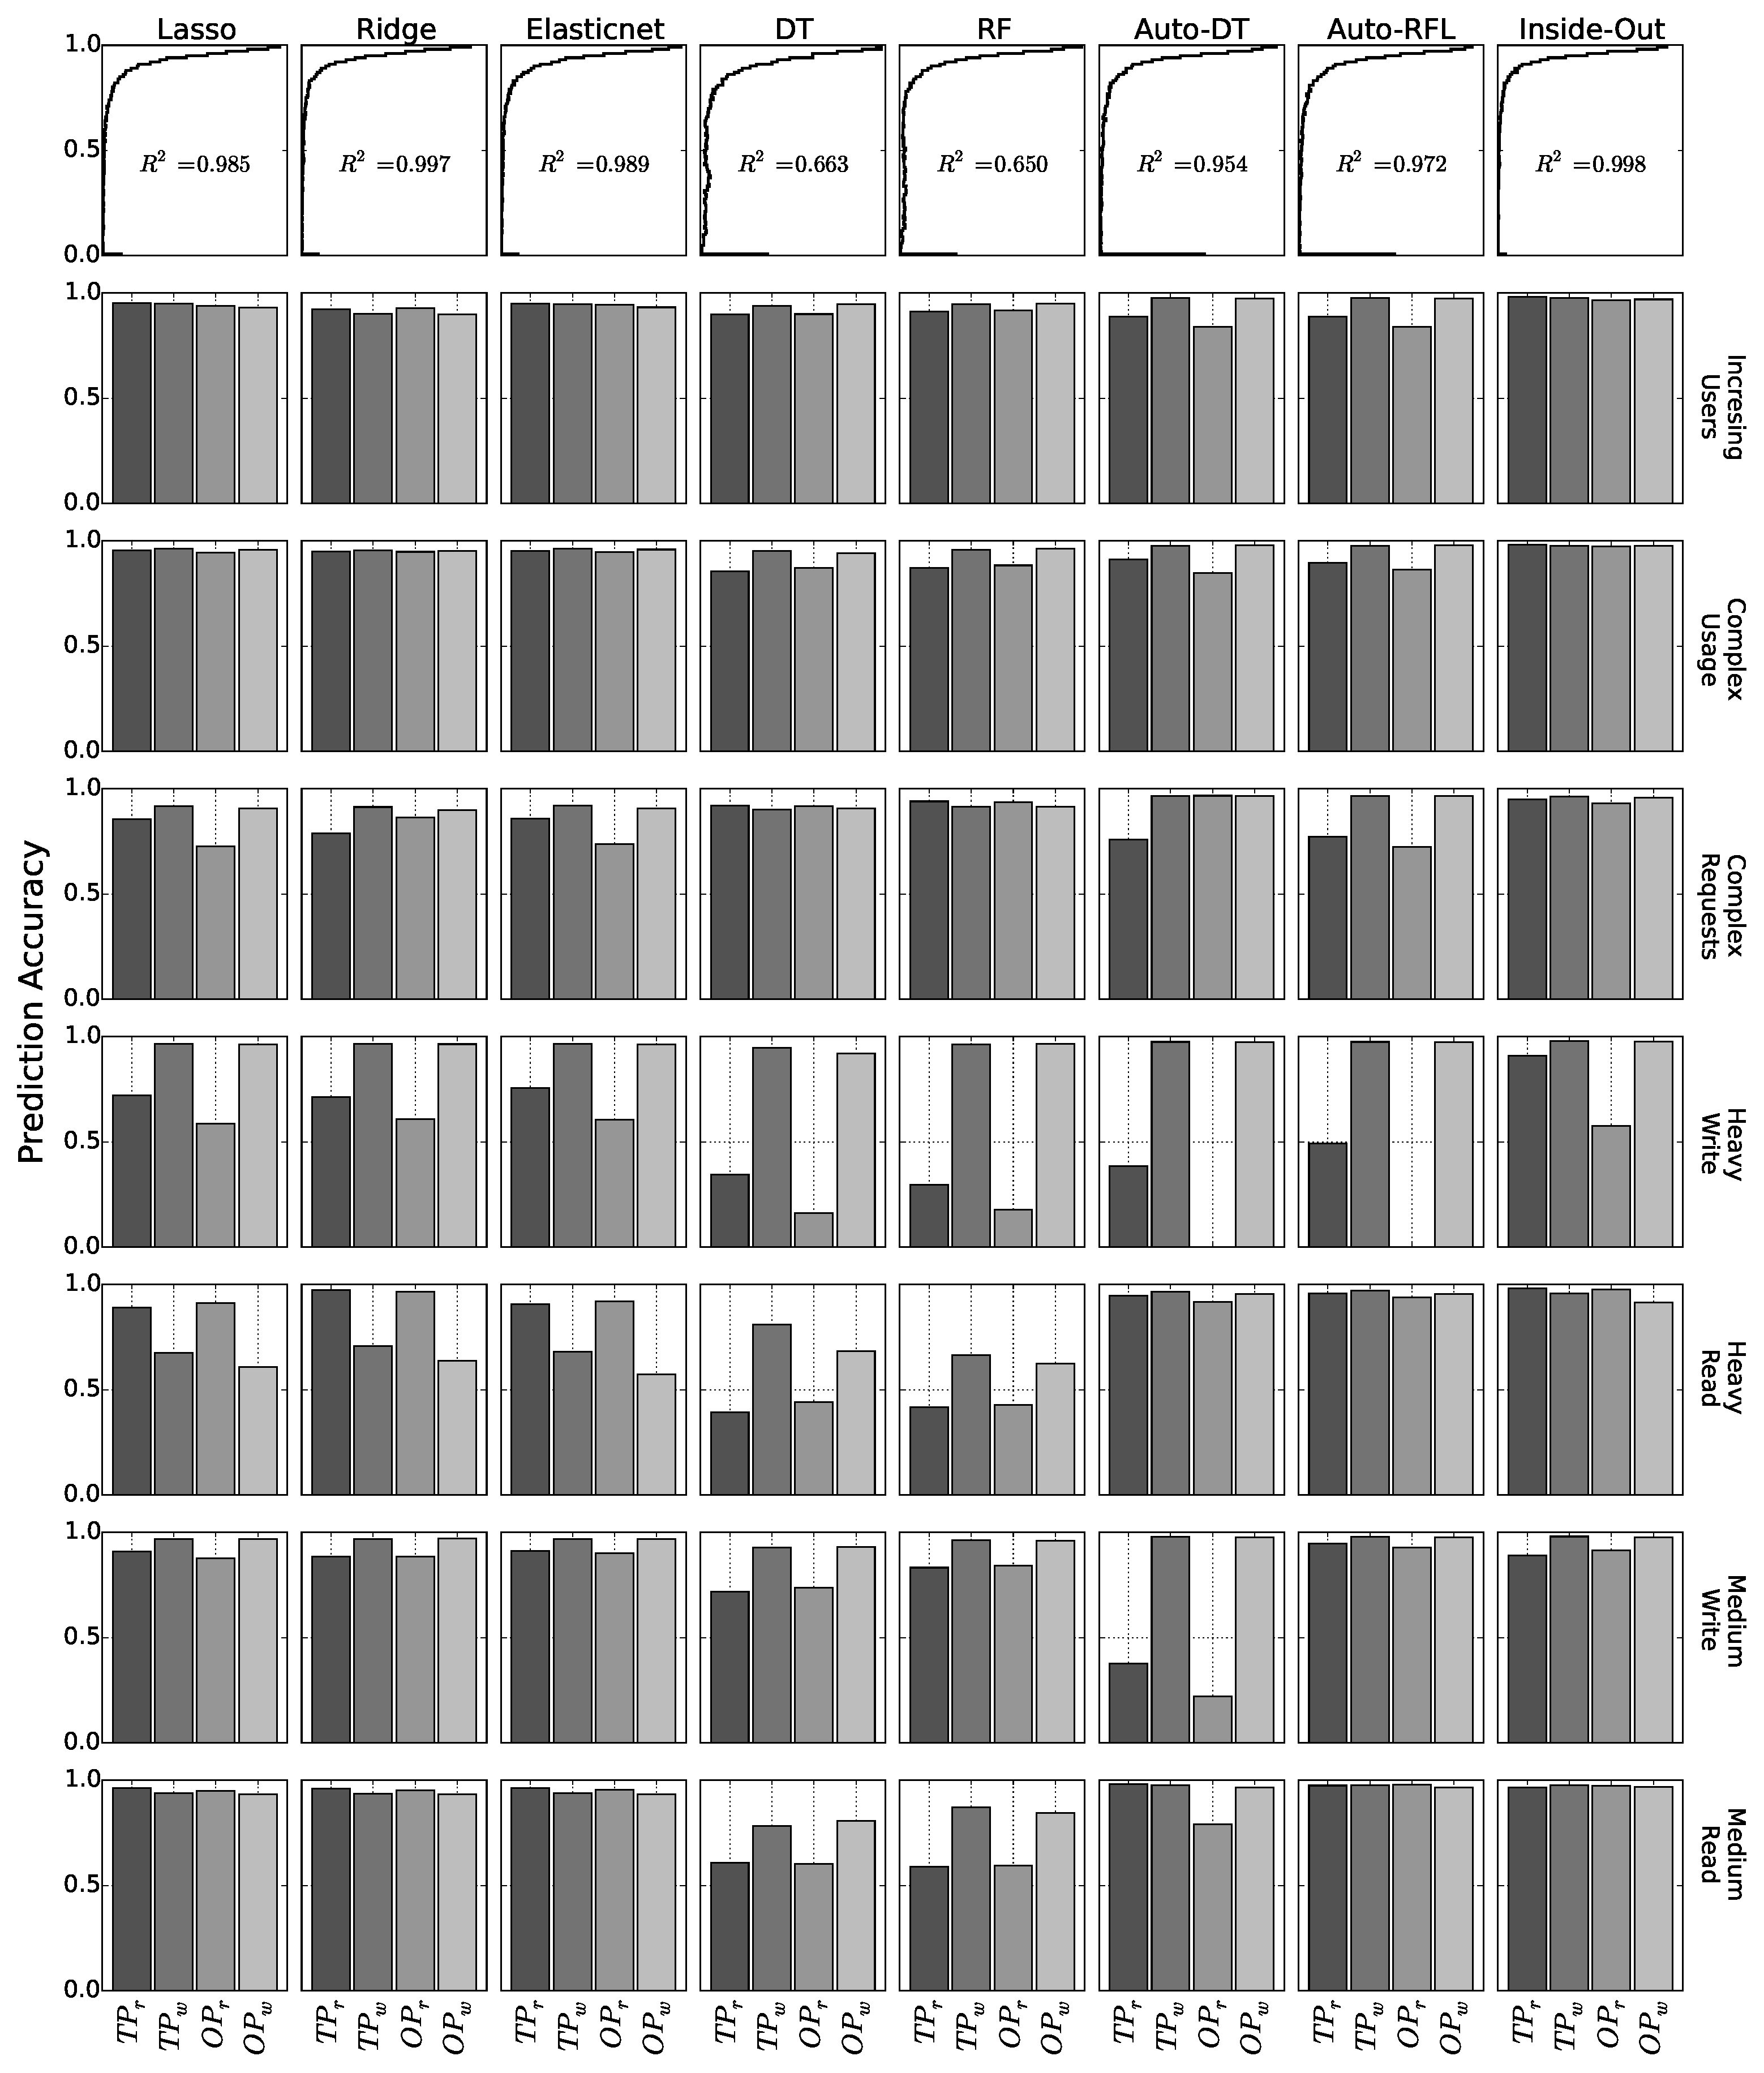
\includegraphics[width=0.9\textwidth]{Chapter-InsideOut/figures/unseen_workload_all_new.eps}
    \caption{Analysis of performance models with diverse workloads. Each bar is the average prediction accuracy. The top row is the probability density function of prediction accuracy for each performance model.}
    \label{fig:changing_workload}
\end{figure}

%\hfill\break

An SDS application needs to handle various request volumes, object/file sizes and different ratios of read/write workloads.
%In practice, it is difficult to obtain a training dataset that includes all access patterns.
First we examine whether Inside-Out can achieve accurate and consistent predictions when workload changes.


\paragraph*{Changing user behavior}
%\textbf{Changing user behavior.}

We increase the number of concurrent clients to stress the Ceph cluster.
%We push the Ceph cluster to a certain limit by increasing the parallelism of clients.
The \emph{\MakeLowercase{\scenarioMU}} scenario changes the number of COSBench clients and the \emph{\MakeLowercase{\scenarioCUB}} scenario increases the worker threads of each client.
As shown in \myfigure{\ref{fig:changing_workload}}, all prediction models perform well. The linear regression technique performs slightly better than the tree-based learning.
The linearly increasing load is well captured by linear models because of proportional change in low-level metrics.
When we switch to the \emph{\MakeLowercase{\scenarioCRB}} scenario, the variable request size slightly changes the behavior of Ceph, affecting prefetching and caching. 
We observe that the linear regression methods (Lasso, Ridge and Elastic Net) show drops in accuracy, e.g. 20\% in the $OP_r$ case; however, Inside-Out 
maintains good accuracy. 
The tree-based learning shows comparable predictions (5-10\% lower) with Inside-Out in these settings.



%\textbf{Complex request behavior.}
%Next, we change the workload from a constant IO request size to variable size.
%In this case, Inside-Out slightly improves the prediction accuracy over Lasso, %and outperforms the three linear models.
%Auto-DT and Auto-RFL show inconsistent prediction result with about 15\% %degradation of accuracy, comparing with the best case.
%One possible expalantion is that some important features filtered by DT and RF 
%are removed.
%Lasso and Elastic Net encounters accuracy drop in the read IOPS prediction


\paragraph*{Varying I/O pattern}

%The workload is a strong performance factor to a storage system \cite{Noorshams2013}.
%The read performance, for example, is affected by the amount of concurrent read or write operations.
Next, we consider workloads with different ratios of read to write operations.
\myfigure{\ref{fig:changing_workload}} shows that varying workload poses a big challenge to performance models. 
The linear regression methods (Lasso, Ridge and Elastic Net) present better prediction accuracy than tree-based models (DT, RL).
In addition, we observe that several models make poor predictions of $TP_r$ and $TP_r$.
The reason is that read behavior is largely affected by \textit{cache}, and large read variance contributes to low prediction accuracy.
Inside-Out performs consistently well, whereas the three linear regression techniques show accuracy drops.
One exception is the $OP_r$ prediction in the \textit{write-intensive} scenario even though $TP_r$ prediction is accurate.
As we will show later in Section~\ref{sec:online_learning}, \emph{over- and under-predictions} cause such behavior. 
The self-learning property of Inside-Out improves its prediction accuracy as it keeps learning the new storage behavior.


\begin{figure}
    \centering
    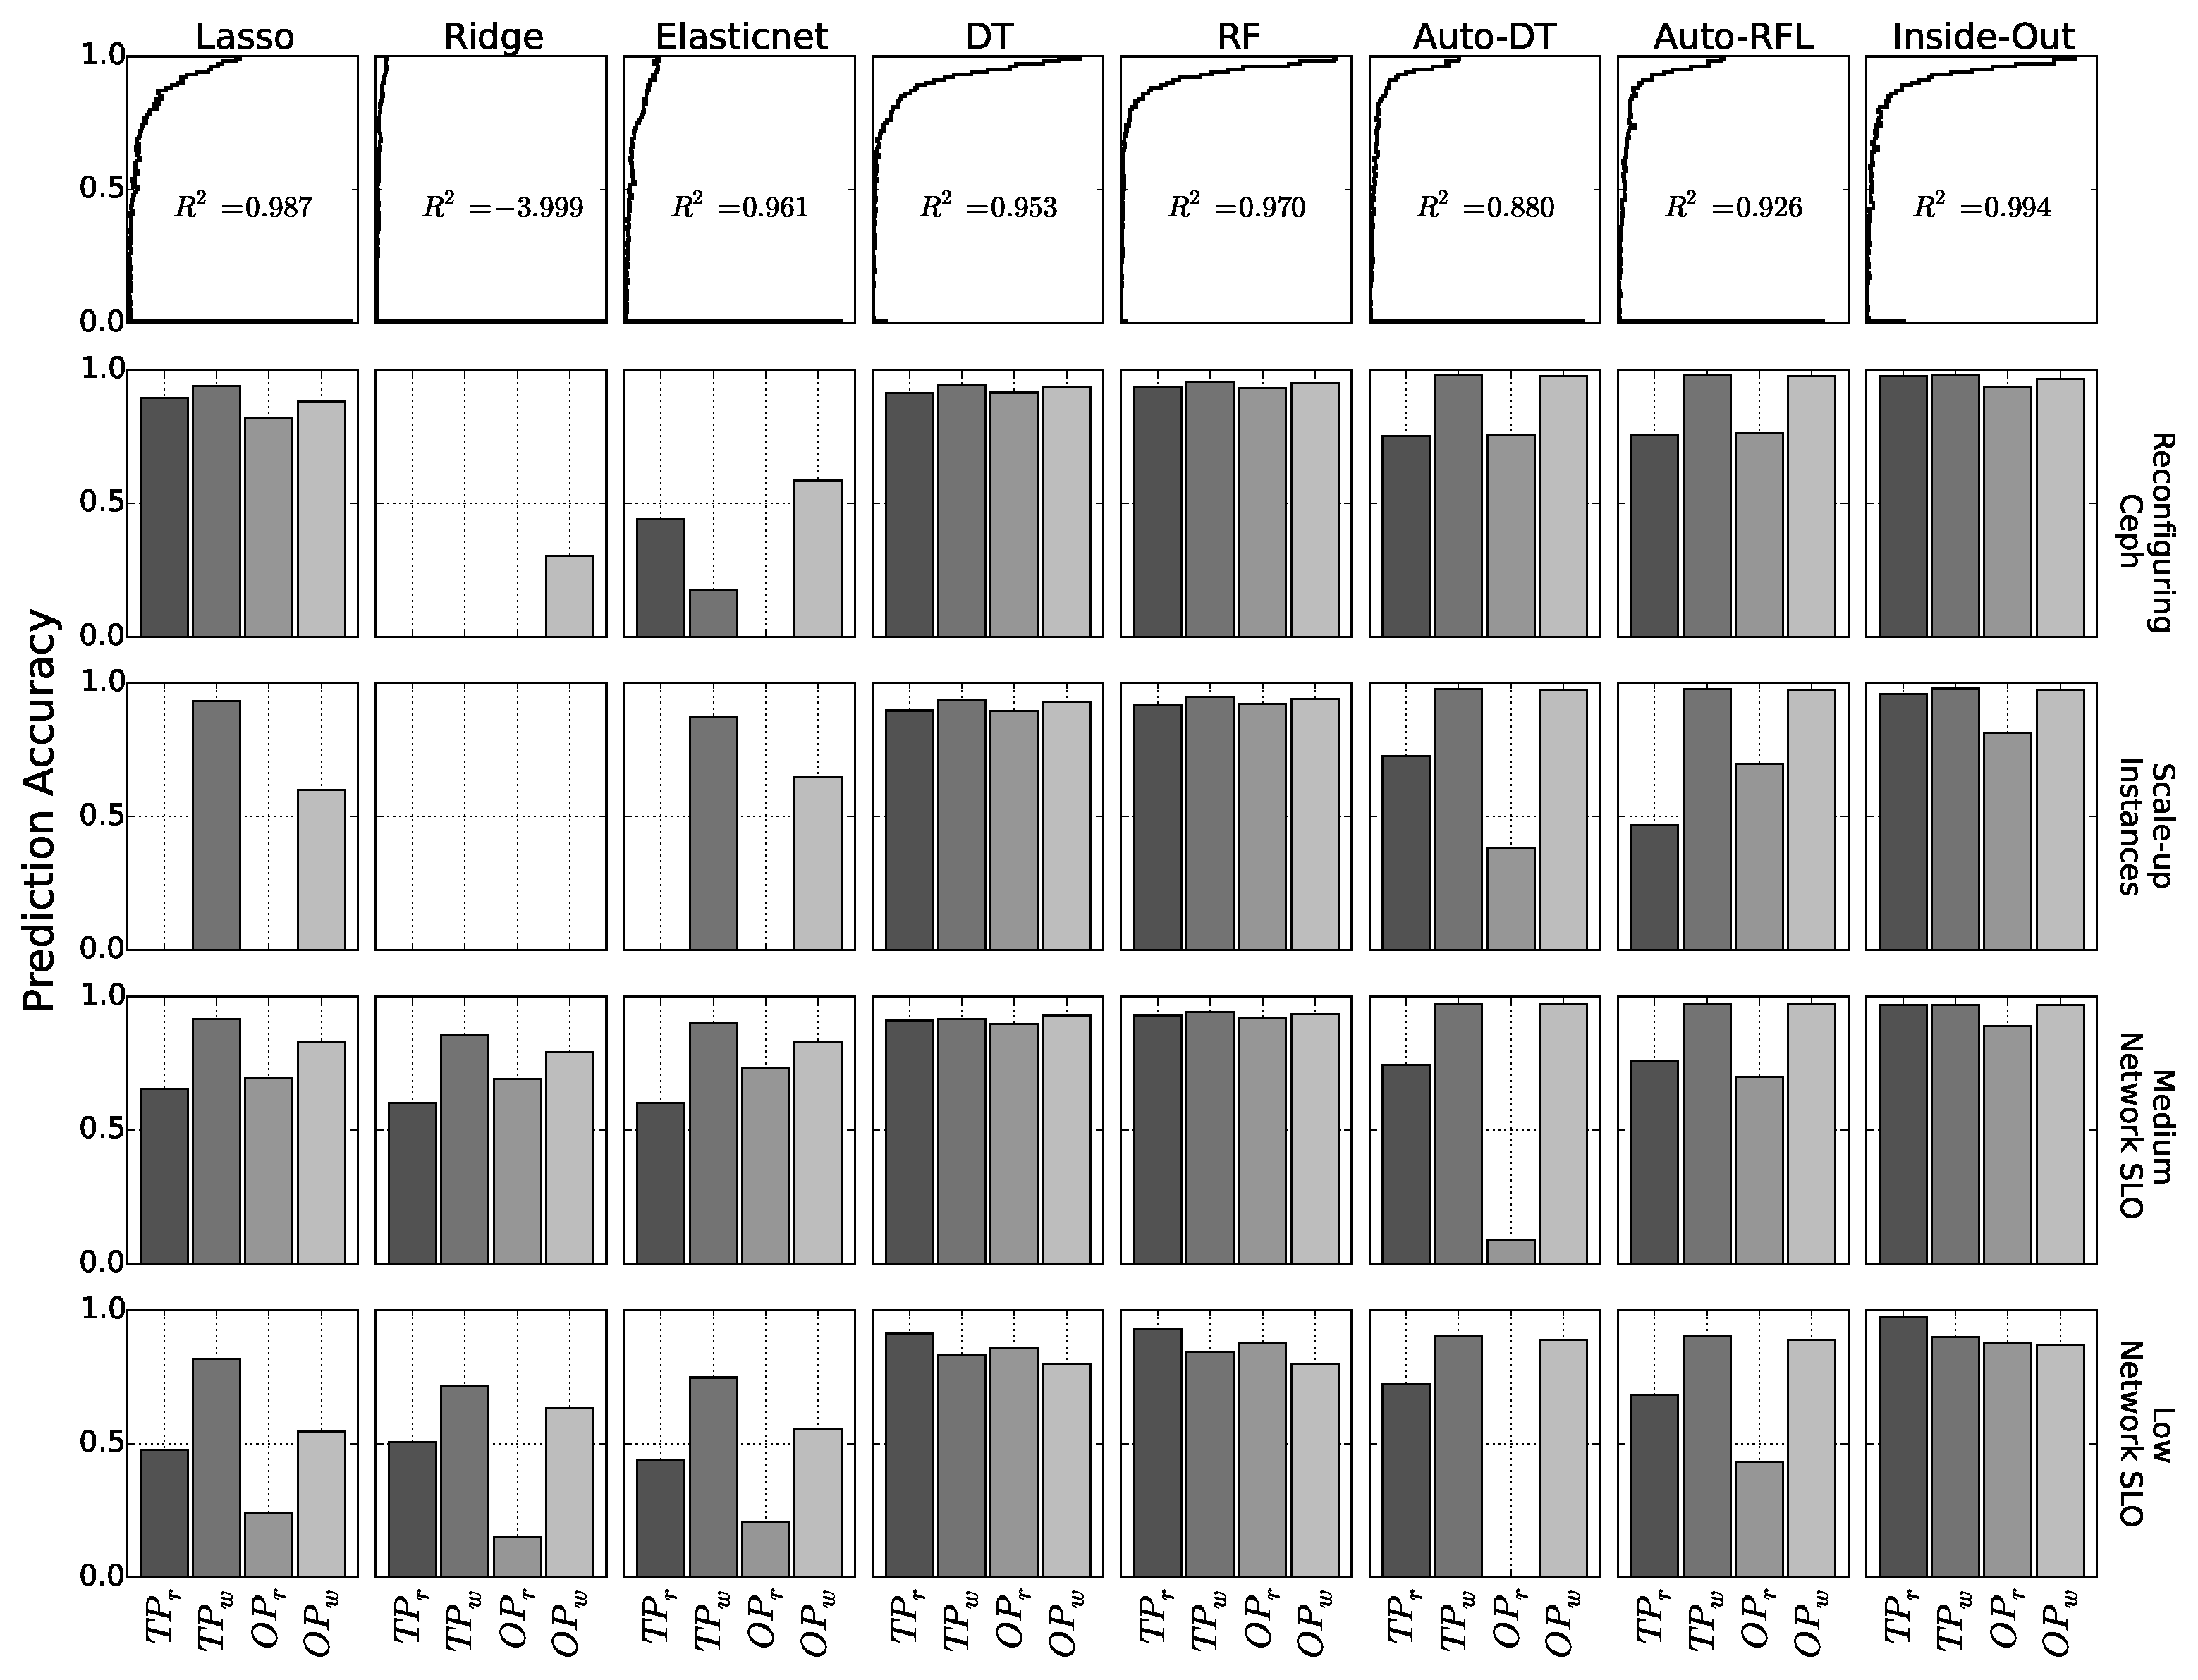
\includegraphics[width=0.9\textwidth]{Chapter-InsideOut/figures/unseen_configuration_all_new.eps}
    \caption{Comparison of performance models when the storage service is reconfigured: Ceph, VMs and network SLOs}
    \label{fig:reconfiguring_storage}
\end{figure}


\paragraph*{Summary}
The linear regression models achieve high prediction accuracy, great goodness-of-fit ($>0.98$) and consistency in prediction 
for many instances (see the distribution of prediction accuracy in \myfigure{\ref{fig:changing_workload}}), but they 
are not consistent across all prediction scenarios.
Inside-Out achieves good prediction accuracy across all cases consistently because the two-level approach 
filters out many irrelevant features in the first step, thereby presenting a smaller relevant feature space to the second step. 
The tree-based learning methods (DT and RF) do not show consistent prediction across all scenarios.
Auto-DT and Auto-RFL, which use DT and RF as the filter algorithms, are not as consistent as Inside-Out.

\vspace{1ex}

%\subsubsection{Reconfiguring Storage}
\subsubsection{Can Inside-Out handle different system configurations?}
\label{sec:unseen_configuration}

We study whether low-level metrics can capture the storage behavior when it is reconfigured by tenants. The results are reported in \myfigure{\ref{fig:reconfiguring_storage}}.


\textbf{Reconfiguring Ceph.}
The first change is to add one extra Ceph monitor daemon. %\chin{which increases the capability to handle a large number of clients.}
Ridge and Elastic Net fail to generate consistent predictions, but Lasso is able to achieve around 80\% to 90\% prediction accuracy.
DT, RF and Inside-Out have very close prediction accuracies, but Auto-DRL and Auto-RFL perform slightly worse in predicting $TP_r$ and $OP_r$.

\textbf{Scale-up instances.}
Increasing CPU and memory allocation to Ceph VM instances improves Ceph's ability to handle more requests.
In this test, we change the instance type from m1.small (1 vCPU, 2GB memory) to m1.medium (2 vCPUs, 4GB memory).
The linear models are unable to predict $TP_r$ and $OP_r$, but Inside-Out's two-level learning performs well by avoiding the overfitting problem. 

\textbf{Network SLOs.}
Here we consider the case where the amount of network bandwidth allocated to Ceph VMs is limited. 
We use Linux network throttling tool \textit{tc} to limit network bandwidth at 500 Mbps and 250 Mbps for medium and low bandwidth SLOs, respectively.
We observe that linear models without the two-level method do not show comparable prediction accuracy across both throughput and IOPS predictions.
The tree-based learning models, on the other hand, achieve 80\% to 90\% accuracy, comparable to Inside-Out.


\textbf{Summary.}
Tree-based learning (DT, RF) models demonstrate promising prediction in terms of prediction accuracy and consistency.
Lasso, Ridge and Elastic Net show inconsistent behavior in the above four scenarios.
Inside-Out, on the other hand, provides consistent predictions and improves Lasso, from 23.9\% to 87.6\% in the extreme case.


\begin{figure}
    \centering
    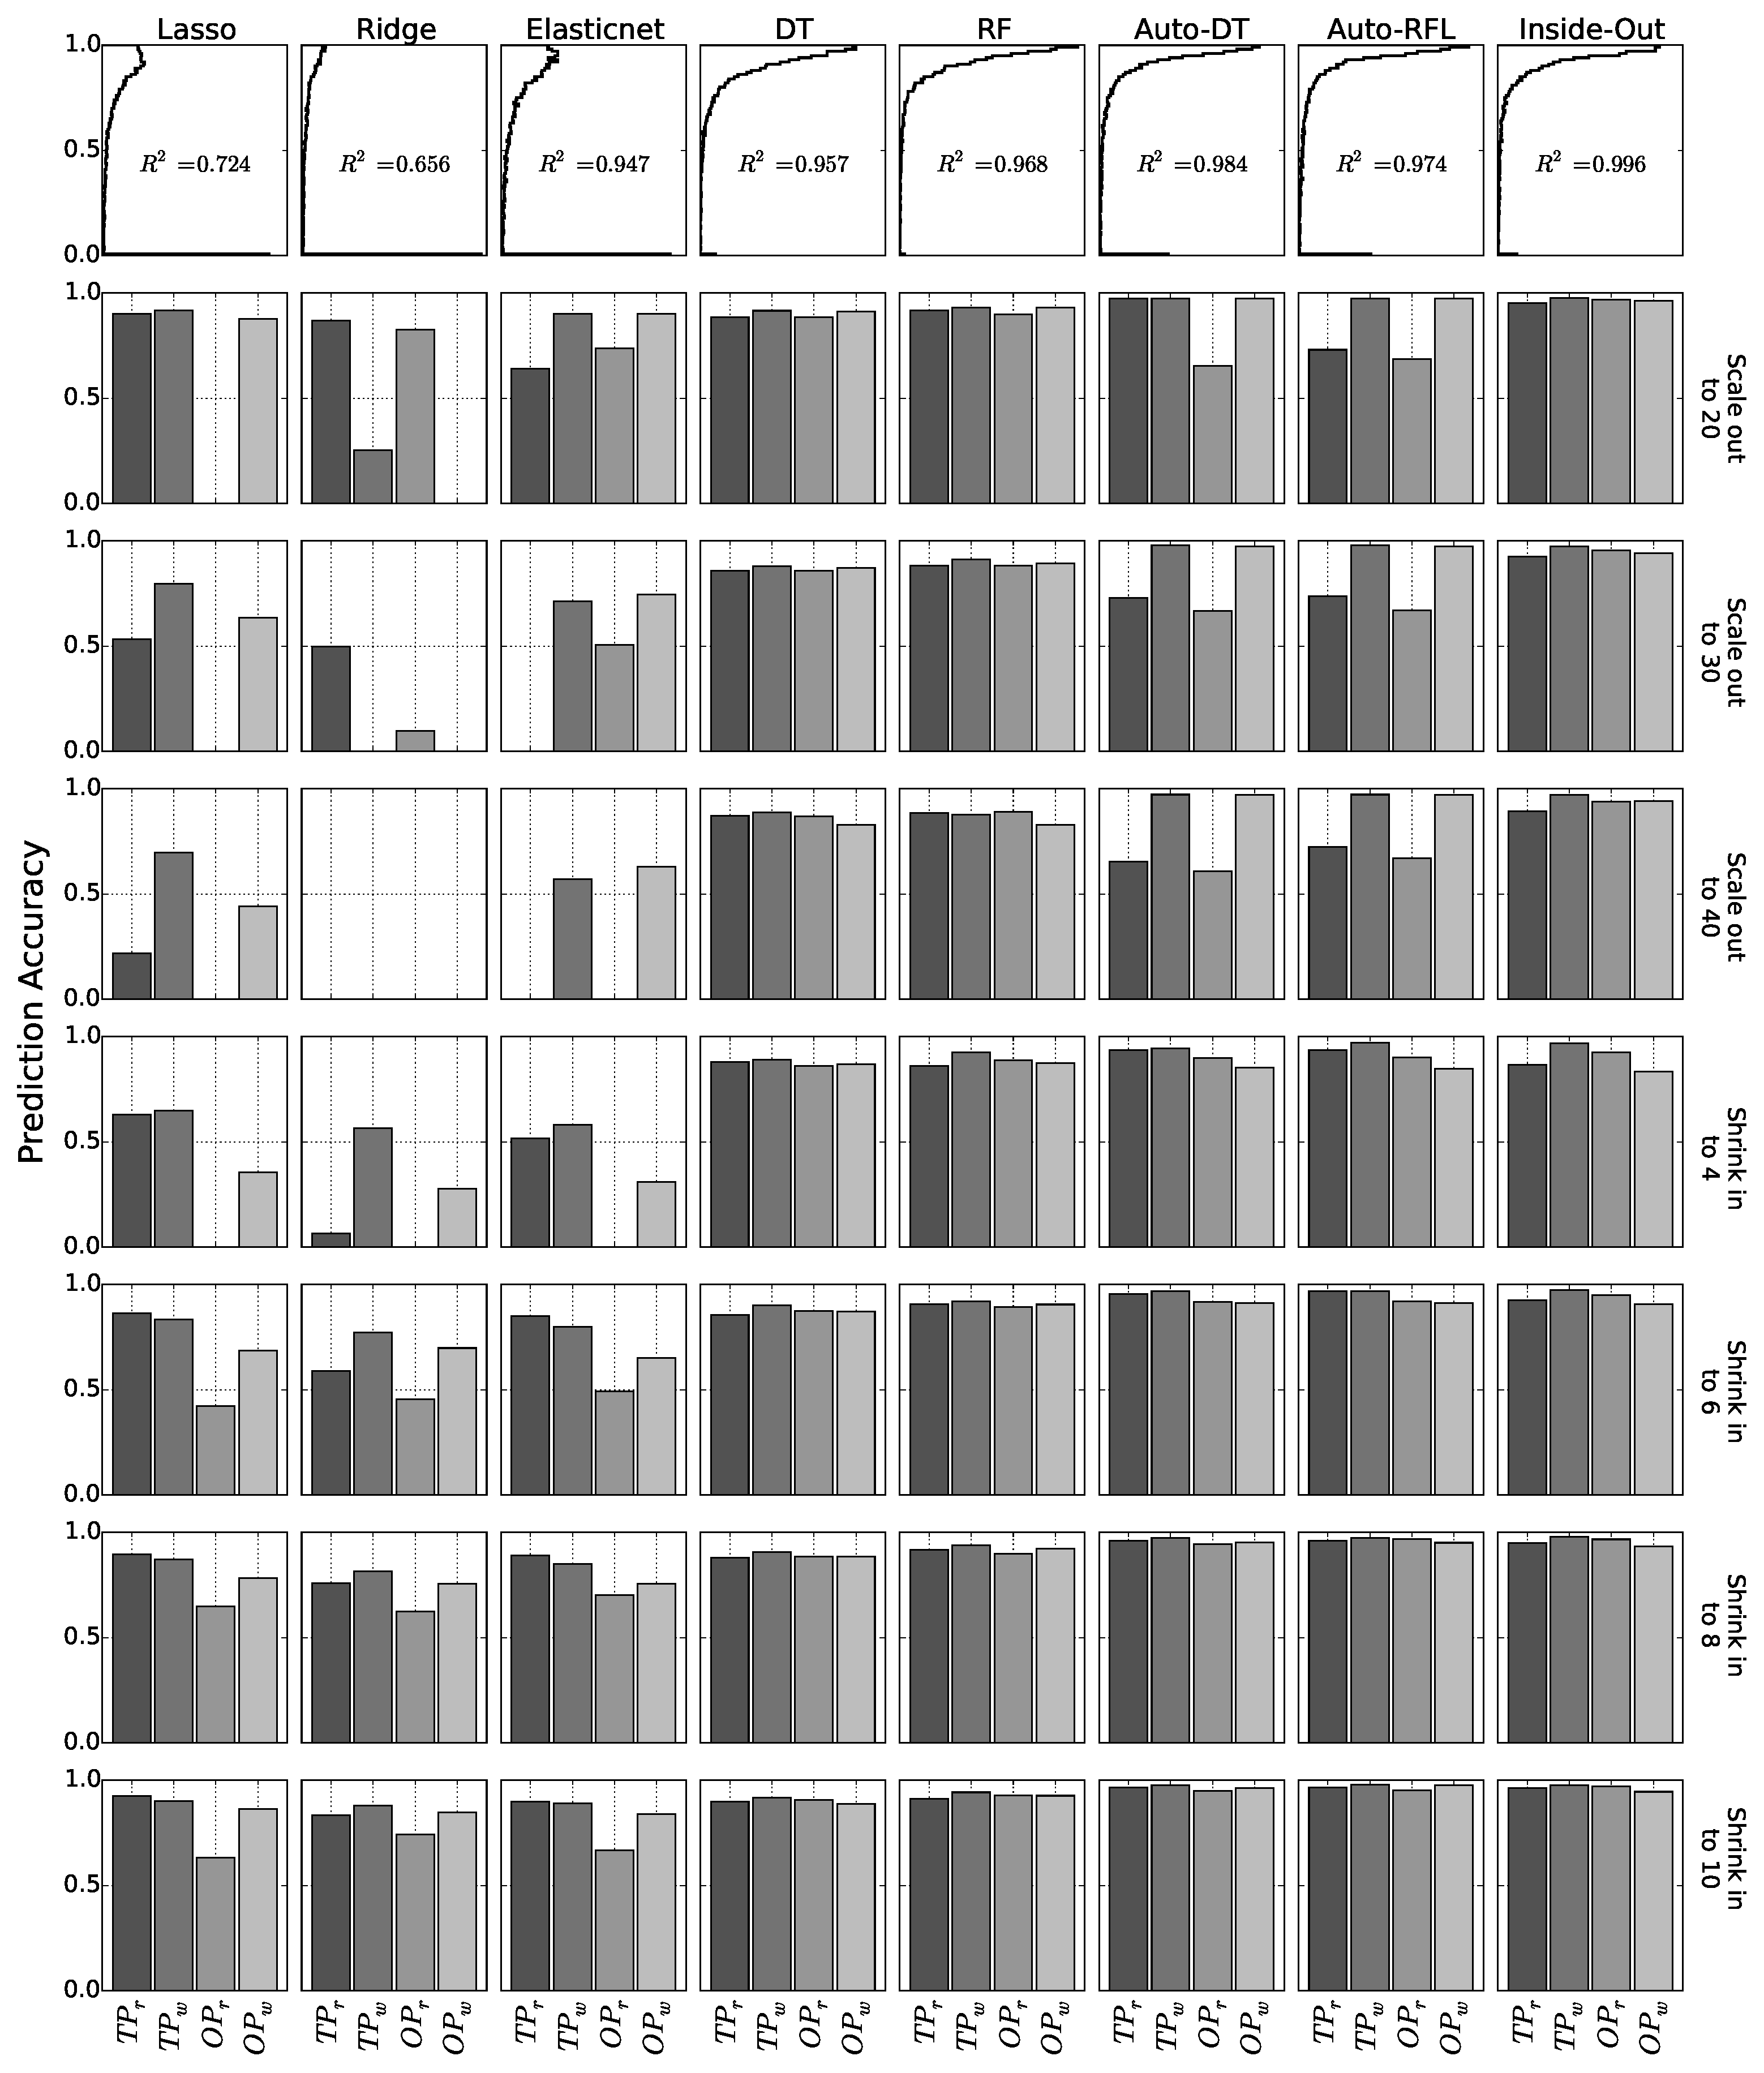
\includegraphics[width=0.9\textwidth]{Chapter-InsideOut/figures/unseen_scale_all_new.eps}
    \caption{Comparison of model performance in the on-demand scaling scenario. In the scale-out scenario, a performance model trained with 10 Ceph nodes is used to predict the performance of Ceph cluster with 20, 30 and 40 nodes.}
    \label{fig:elasticity}
\end{figure}


\subsection{Prediction Performance in a Multi-tenant Cloud}

This section examines the modeling performance of Inside-Out.
We first evaluate whether Inside-Out is able to extrapolate
performance of a larger Ceph cluster. 
Next, we evaluate how Inside-Out performs
when systems are subject to performance interference.

\subsubsection{Elastic Storage (On-demand Scaling)}
\label{sec:scaleout_prediction}

A storage service needs to grow or shrink its capacity on demand.
We evaluate Inside-Out's ability to capture the storage behavior at different system scales.
As shown in \myfigure{\ref{fig:elasticity}}, we use training data collected from 
4, 6, 8, and 10 nodes, and then predict the performance of 20, 30, and 40 nodes.
We also evaluate prediction accuracy in the \emph{shrink-in} scenario.
For both read and write throughput predictions, the linear models exhibit high variance.
In the $OP_r$ and $OP_w$ cases, the prediction results are not even comparable to the other methods.
Inside-Out, on the other hand, helps mitigate this issue, and achieves more than 90\% accuracy.
With increasing sizes of the storage, the prediction accuracy decreases because the prediction target 
becomes increasingly different from the training data.
Running a benchmark test against a very large system is time-consuming.
Here we demonstrate that Inside-Out can predict performance for systems that are 
four times larger than the system for which training data was collected.
%Due to resource limitations, we cannot show the upper bound of the largest system size that we can predict.
%However, we believe the upper bound can increase as the performance model keeps learning the system behavior.

\begin{figure}
    \centering
    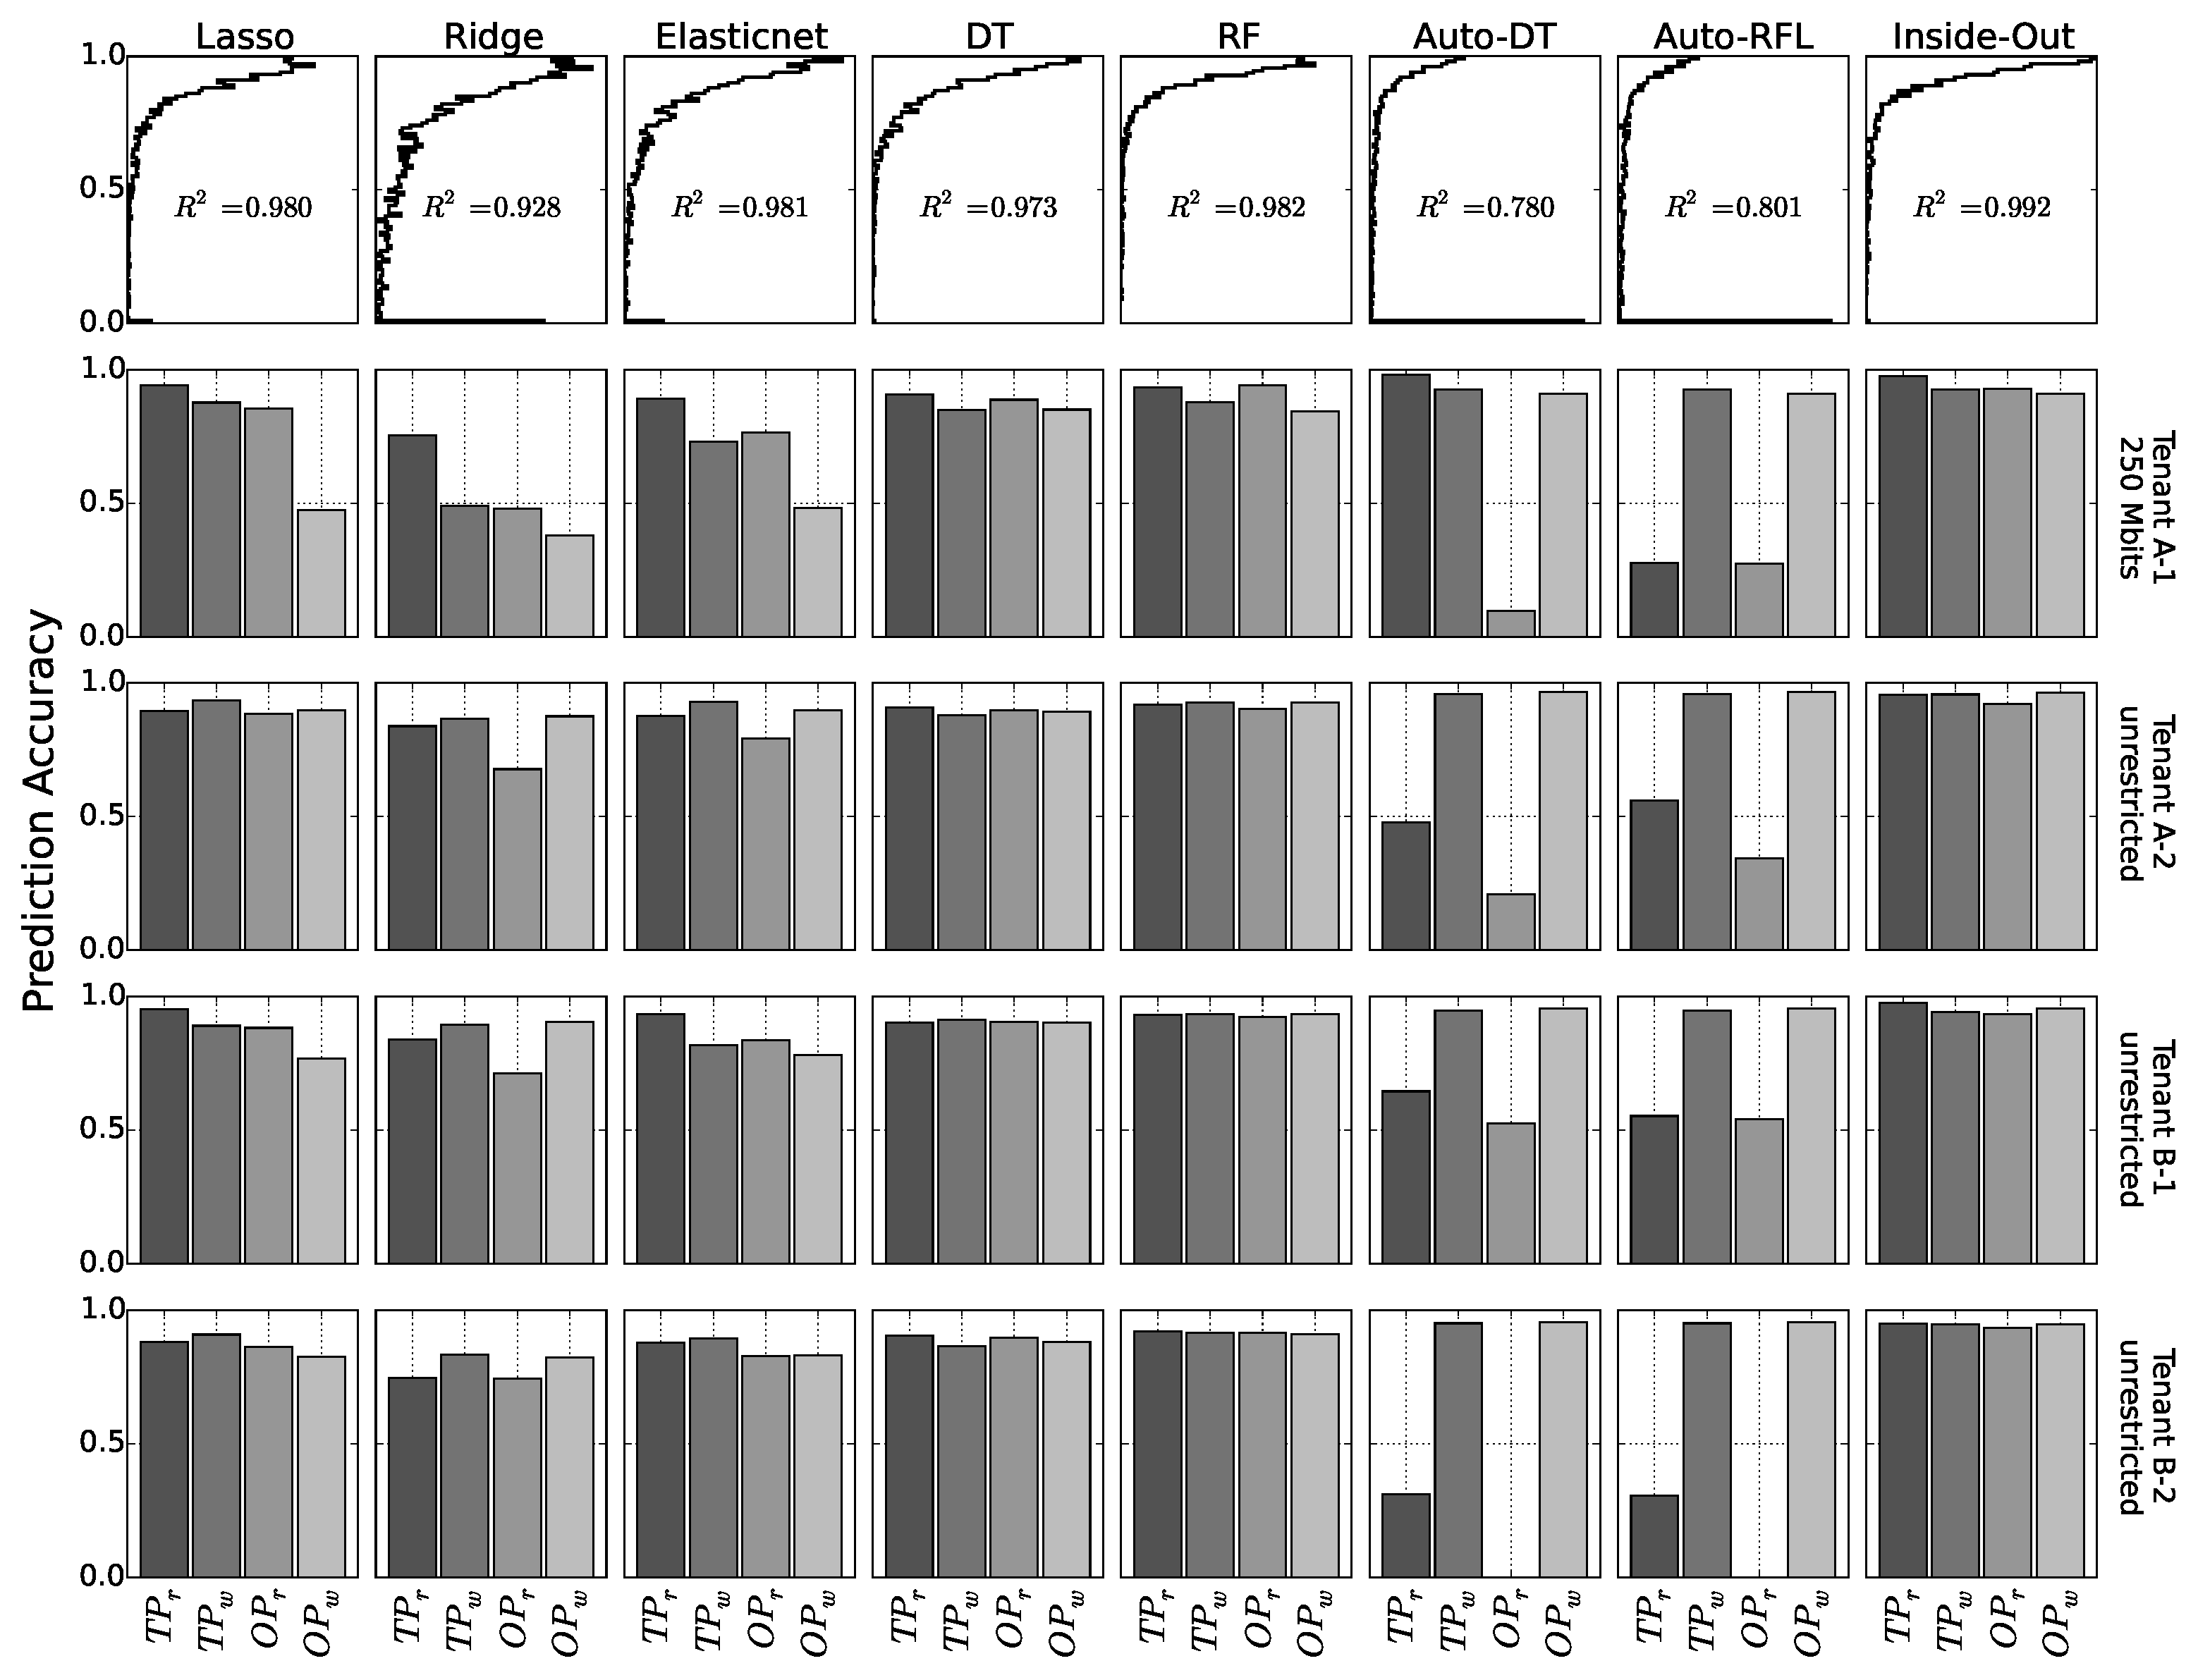
\includegraphics[width=0.9\textwidth]{Chapter-InsideOut/figures/multi_tenancy_all_new.eps}
    \caption{Prediction accuracy in a multi-tenancy scenario. Tenant A-1 is co-located with Tenant B-2. Tenant A-1 is throttled at 250Mbps. Tenant B-1 and B-2 are co-located without any traffic throttling.}
    \label{fig:multi_tenancy}
\end{figure}


\begin{figure*}
    \centering
    \includegraphics[width=0.9\textwidth]{Chapter-InsideOut/figures/real-world_tp_read.pdf}
    \caption{Application of Inside-Out to real time prediction of read throughput on a 10-node Ceph cluster.  Inside-Out starts from a simple prediction model trained by our collected benchmarking data.  Inside-Out keeps learning the storage behavior while improving prediction accuracy over time.}
    \label{fig:real_workload}
\end{figure*}


\subsubsection{Multi-Tenancy}
 
Next we evaluate Inside-Out's ability to adapt to performance interference among storage tenants.
We consider two cases for this evaluation. 
Each tenant runs a Ceph cluster with 10 OSDs separately, but tenants share the same 10 physical machines.
In the first case, we restrict the bandwidth of only the first tenant at 250Mbps.
%Two tenants compete for resources and \chin{\textbf{Tenant A-1}} has lower bandwidth SLO.
In the second case, we run two concurrent Ceph clusters but without network throttling.
\myfigure{\ref{fig:multi_tenancy}} shows that most prediction models are able to achieve more than 80\% accuracy.
The linear models like Ridge and Elasticnet yield lower prediction accuracies in some cases; however, Inside-Out performs well consistently.
Performance interference is challenging for a performance model designed for an isolated environment.
This evaluation demonstrates that the low-level performance metrics are good proxies for measuring
the end-to-end storage performance, even in a shared SDS environment.
%These metrics are able to reflect the behavior changes in the storage system.

%low-level performance feature selection approach is effective in capturing end-to-end performance, even under high storage interference.
%This property is important to SDS because it can help guarantee reliable end-to-end performance in a shared SDS environment.



\begin{comment}
\begin{figure*}
    \centering
    \includegraphics[width=0.9\textwidth]{figures/synthetic.eps}
    \caption{An online prediction scenario about six-hour long workload.  This synthetic workload is composed of 360 stages and each stage uniformly selects parameters such as workload types, request sizes and the number of clients.  The average stage duration is 60 seconds with standard deviation 20 seconds.}
\end{figure*}
\end{comment}

\begin{comment}
\begin{figure*}
    \centering
    \begin{subfigure}[b]{0.45\textwidth}
        \includegraphics[width=\textwidth]{figures/synthetic_read.eps}
        \caption{Read Throughput}
        \label{fig:synthetic_read}
    \end{subfigure}
    ~ %add desired spacing between images, e. g. ~, \quad, \qquad, \hfill etc.
      %(or a blank line to force the subfigure onto a new line)
    \begin{subfigure}[b]{0.45\textwidth}
        \includegraphics[width=\textwidth]{figures/synthetic_write.eps}
        \caption{Write Throughput}
        \label{fig:synthetic_write}
    \end{subfigure}
    \caption{An online prediction scenario about six-hour long workload.  This synthetic workload is composed of 360 stages and each stage uniformly selects parameters such as workload types, request sizes and the number of clients.  The average stage duration is 60 seconds with standard deviation 20 seconds.}
    \label{fig:synthetic_workload}
\end{figure*}
\end{comment}

%\subsection{Synthetic Workload}
\subsection{Online Self-Learning}
\label{sec:online_learning}

%Our goal is to apply Inside-Out to an online system so that SDS providers can guarantee the performance of a storage service hosted on their SDS platform.
%To evaluate this potential, 
Next, we create several synthetic workloads with mixed read/write ratios.
This synthetic workload spans 12 hours with 720 stages.
Each stage is 60-second long on average, with a standard deviation of 20 seconds.
We run four COSBench virtual machines for benchmarking and up to eight threads per COSBench client, with 10 Ceph OSDs and one monitor daemon.
We use Inside-Out to build an initial performance model with the training dataset described in Section~\ref{sec:dataset}.
\myfigure{\ref{fig:real_workload}} shows the prediction result for read throughput.
We can observe that the generated model can capture the overall trend, but suffers from over and under predictions.
This is because our training dataset is generated from a relatively clean environment, \ie the OS memory is flushed before any benchmarking process.
However, in the online prediction setting, cache is continuously consumed by non-stop client requests, which 
causes the real time storage behavior to be different from the training dataset.
With continuous monitoring of the performance of the storage service, 
we use Inside-Out to generate a new performance model at the sixth hour.
\myfigure{\ref{fig:real_workload}} shows that Inside-Out learns the new storage behavior and therefore, 
the over- and under-prediction issues are greatly mitigated.
%This evaluation demonstrates the potential of Inside-Out when applying it in an online system.
By continuously learning the storage behavior, SDS can accurately capture performance changes and therefore is able to provide reliable storage service.

%the problems due to over- and under-predictions are greatly mitigated.
%This evaluation demonstrates how Inside-Out can be used to continuously learn the storage behavior in an online system.


\begin{figure}
\centering
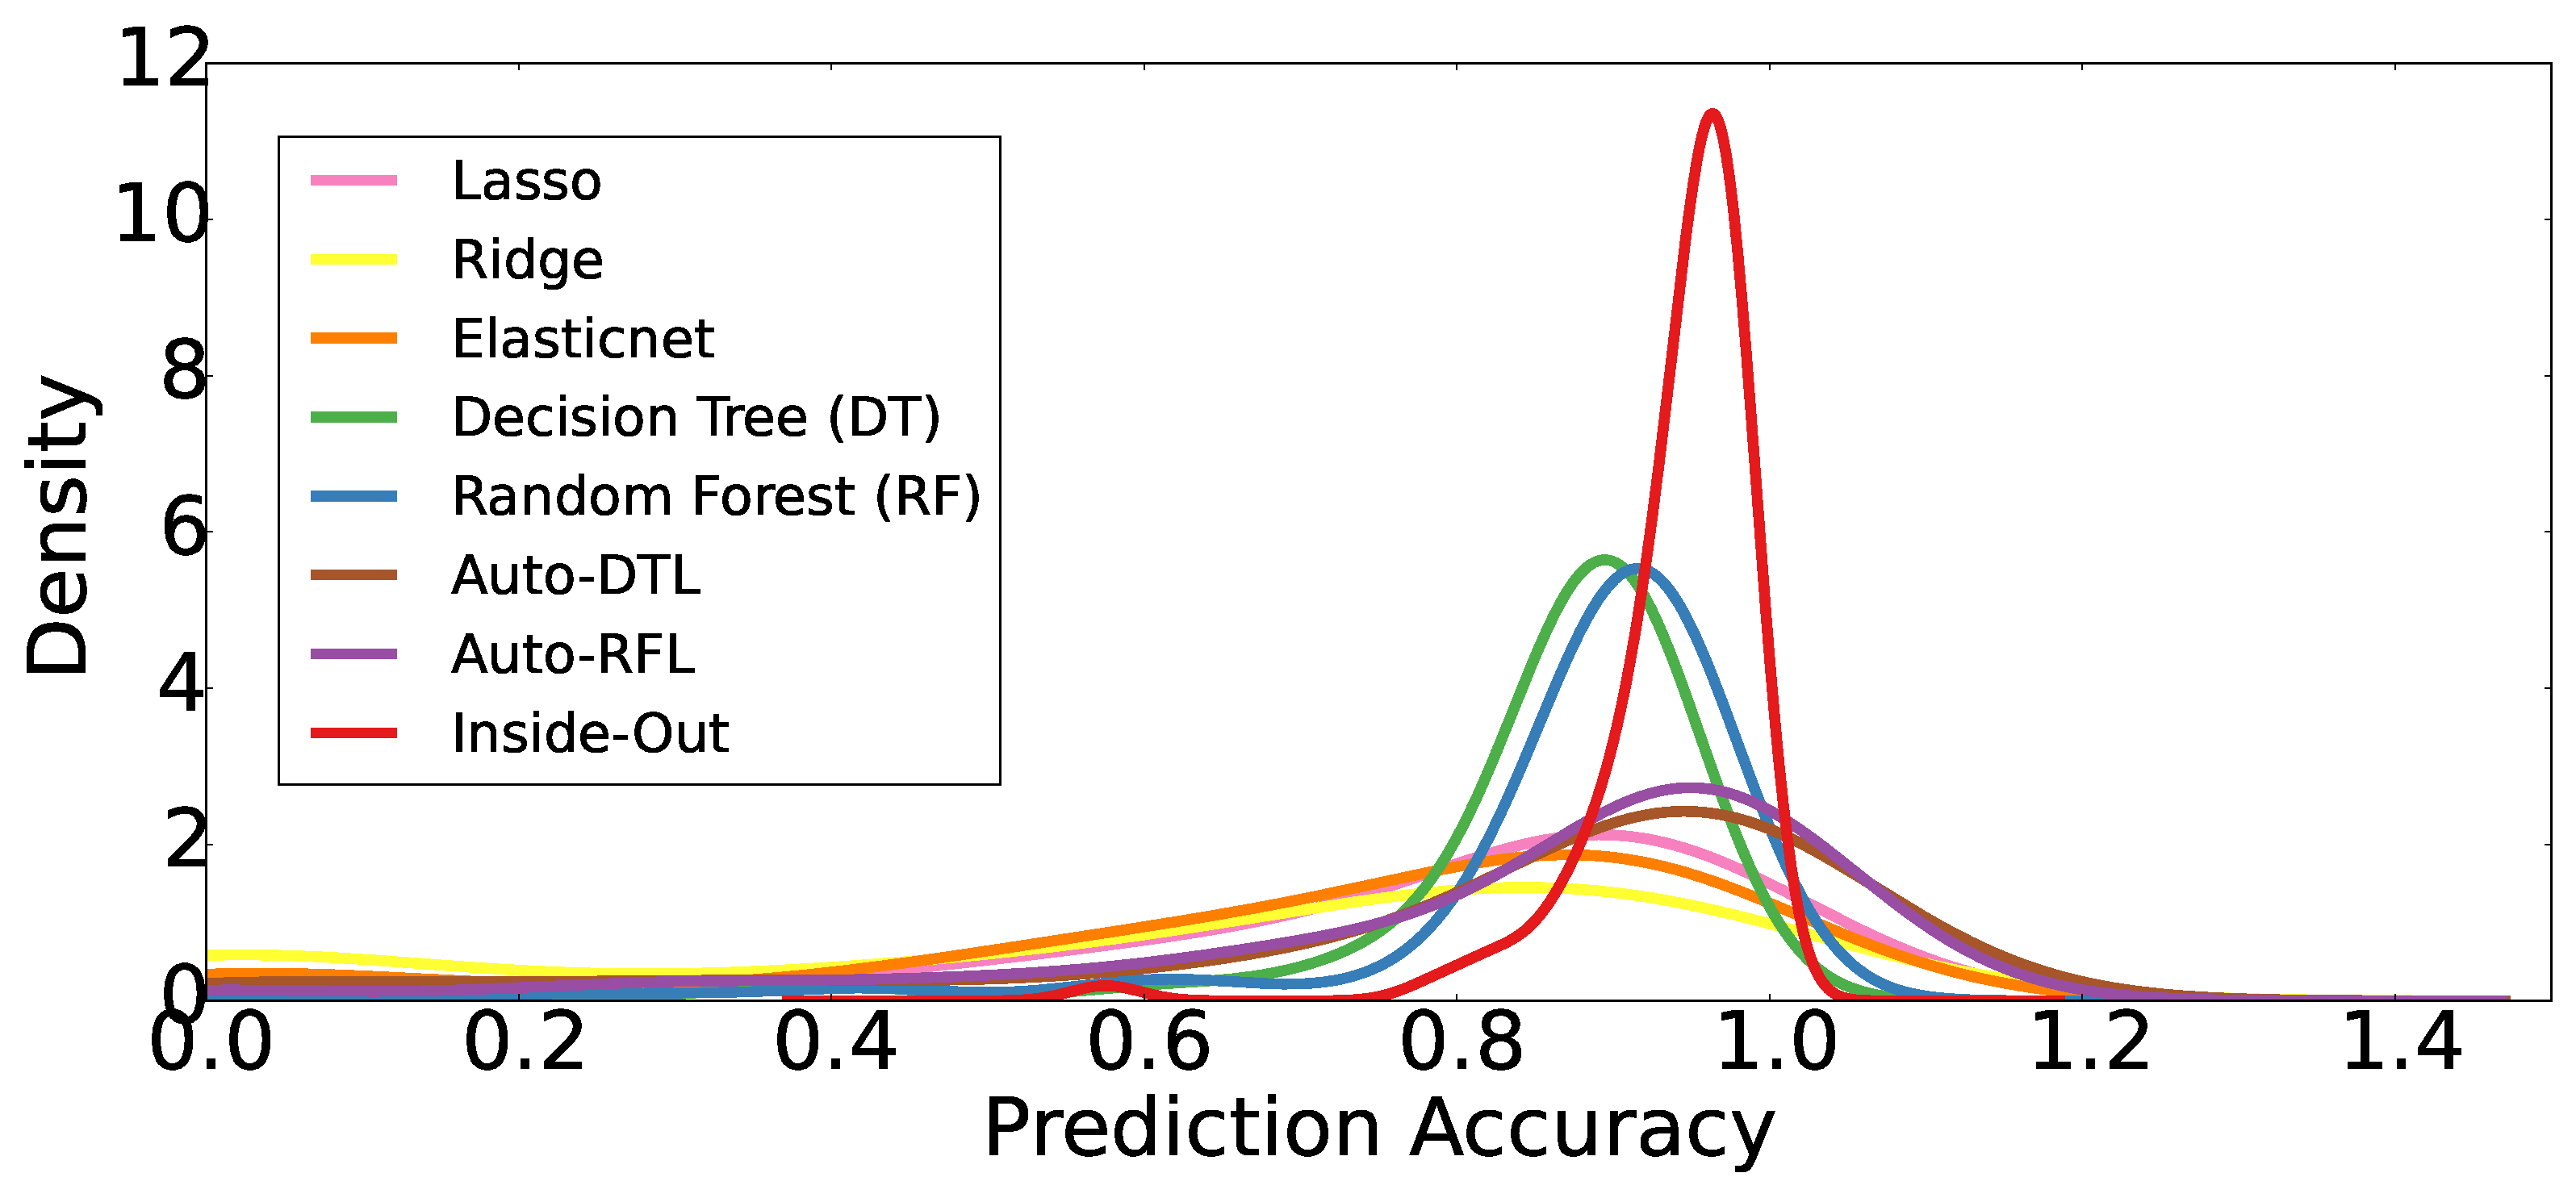
\includegraphics[width=0.9\textwidth, keepaspectratio]{Chapter-InsideOut/figures/aggregate_median.eps}
\caption{Kernel density function of prediction accuracy from \myfigure{\ref{fig:changing_workload}} to \myfigure{\ref{fig:multi_tenancy}}.  Each colored line represents the density function of a modeling approach.  Inside-Out is more consistent and accurate across almost every prediction case.}
\label{fig:aggregate}
\end{figure}


\vspace{1ex}
\subsection{Discussion}
We have shown that low-level performance metrics are useful to predict end-to-end throughput and IOPS.
%We applied Inside-Out to latency prediction and observe large variance and inconsistency.
%\chin{One} possible explanation is insufficient features and high variance in latency.
%The \chin{collected} low-level metrics are related to utilization, and these metrics might not provide enough information to fit a good model for predicting latency.
%Common approaches usually require request-level information \cite{Wang2004}.
%We need to further investigate latency prediction with other alternative generic low-level performance metrics.
Our evaluation has shown that low-level performance metrics are good indicators of end-to-end throughput and IOPS. 
Most existing performance models exhibit an inconsistent prediction behavior in the presence of diverse storage scenarios, 
such as changing workload, storage reconfigurations,
growing/shrinking storage, and multi-tenancy environments.
Our proposed two-level learning method can greatly improve prediction accuracy and yield consistent behavior.
Machine learning provides powerful tools, but they need to be used intelligently to achieve the best prediction accuracy. 
\myfigure{\ref{fig:aggregate}} shows the kernel density function of prediction accuracy across all prediction scenarios.
Inside-Out is a clear winner in terms of accuracy and consistency. 
More importantly, Inside-Out is able to learn new storage behavior, thereby enabling the performance model to adapt to the complex SDS environment.





%\section{Related Work}
\label{sec:related_work}

\begin{itemize}
\item
  Characterizing application
\item
  Analyzing the energy-time trade-off in high-performance computing
  applications
\item
  Dynamically Controlling Node-Level Parallelism in Hadoop
\item
  Data-Driven Performance Modeling
\item
  Model Building

  \begin{itemize}
  \item
    Inside-out
  \end{itemize}
\item
  Configuration Recommendation
\item
  Parameter Tuning

  \begin{itemize}
  \item
    Selfish
  \item
    Dynamically Controlling Node-Level Parallelism in Hadoop
  \end{itemize}
\item
  Storage configurations
\item
  Cloud configurations

  \begin{itemize}
  \item
    Earnest
  \item
    CherryPick
  \end{itemize}
\item
  Search Algorithms
\item
  Random Search
\item
  Coordinate Descent
\item
  Genetic Algorithm
\item
  Bayesian Optimization
\end{itemize}
%\section{Conclusion}
\label{sec:conclusion}

The decoupled Hadoop model is flexible and much more preferable in many scenarios.
However, existing Hadoop schedulers do not consider this model and hence the scheduling method fails to optimize the system throughput.
Our flow scheduling method uses the penalty cost for task assignments in order to increase the processing flow rate on computing facilities.
We encode this problem as the min-cost flow problem and then we can obtain the optimal assignment.
We have implemented a pluggable Flow Scheduler for Hadoop YARN and it supports the latest version of Hadoop.
Our experiment results have shown that our flow scheduling can greatly improve the system throughput by about 30\% so as to eliminate stragglers.
These results support that the proposed flow scheduling can maintain the flow rate of processing.

Flow scheduling seems efficient for the decoupled model, but there still remains large space to improve.
For our current implementation, Flow Scheduler requires job profile and machine profile, which is not practical.
We believe we can estimate the flow demand of tasks and the flow capability of facilities at runtime.
A naive approach is to sample the flow demand of a task and then use this information to decide the cost of the remaining tasks of the same job.
Another approach is to monitor the flow rate of tasks so that we can adjust the penalty cost dynamically.
We can also decide the flow capability of facilities in a similar way.
Overall, we are positive about flow scheduling but more extensive evaluations have to be conducted before we can conclude.
